\chapterimage{Pictures/chap05/measure-one180-1260x630.png}
\chapter{颜色和辐射学}\label{chap:颜色和辐射学}
\setcounter{sidenote}{1}

为了精确描述光是怎样被表示和采样以计算图像的,
我们必须首先建立一些\keyindex{辐射学}{radiometry}{}的背景——
\keyindex{电磁辐射}{electromagnetic radiation}{}在环境中的传播研究。
渲染中尤其感兴趣的是\keyindex{波长}{wavelength}{}($\lambda$)大约在
380nm到780nm的电磁辐射\sidenote{译者注:nm即长度单位纳米。$1$纳米=$10^{-9}$米。},
主要是人眼可见光\footnote{可感知波长的完整范围稍微超出了该区间,
但眼睛在这些波长上的敏感性低了许多量级。当绘制光谱曲线时常把范围360-830nm用作保守边界。}。
较短波长($\lambda\approx400\text{nm}$)是偏蓝色的,
中间波长($\lambda\approx550\text{nm}$)是绿色的,
而较长波长($\lambda\approx650\text{nm}$)是红色的。

本章中,我们将介绍描述电磁辐射的四个关键量:
\keyindex{通量}{flux}{}、\keyindex{强度}{intensity}{}、
\keyindex{辐照度}{irradiance}{}和\keyindex{辐亮度}{radiance}{}。
这些辐射量每一个都由它们的\keyindex{光谱功率分布}{spectral power distribution}{}(SPD)——
描述在各波长上的光量关于波长的函数。
pbrt中用定义于\refsec{光谱表示}的类\refvar{Spectrum}{}来表示SPD。

\section{光谱表示}\label{sec:光谱表示}

真实世界物体的SPD可能极其复杂;
\reffig{5.1}展示了荧光灯发光的频谱分布和柠檬皮反射率的频谱分布图。
用SPD做计算的渲染器需要紧实、高效且准确的方式表示像这样的函数。
实践中,可能需要在这些特性间作取舍。
\begin{figure}[htbp]
    \centering
    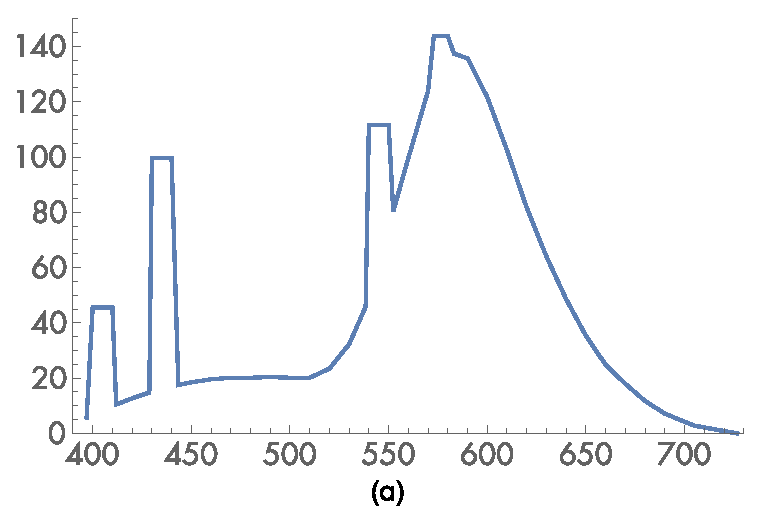
\includegraphics[width=0.45\linewidth]{chap05/fluorescent-spd.eps}\,\nolinebreak
    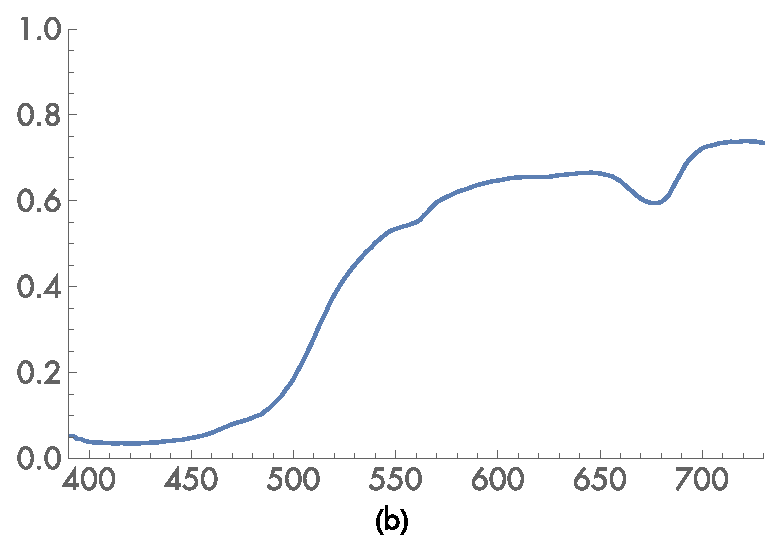
\includegraphics[width=0.45\linewidth]{chap05/lemonskin-spd.eps}
    \caption{(a)荧光灯的频谱分布和(b)柠檬皮的反射率。
    波长400nm左右是偏蓝光,而波长中段是绿色和黄色,波长700nm左右是红光。
    荧光灯的SPD甚至比这里展示的更加尖锐,SPD可归入到10nm范围内;
    它实际上是在单个离散频率上发出大量光。}
    \label{fig:5.1}
\end{figure}

研究这些问题的一般框架可以基于寻找
优良\keyindex{基函数}{basis function}{}以表示SPD的问题来开发。
基函数背后的思想是将可能的SPD函数的无限维空间映射到系数$c_i\in\mathbb{R}$的低维空间。
例如,一个平凡的基函数是常函数$B(\lambda)=1$。
任意SPD可以用等于其平均值的单个系数$c$以该基表示,
这样其近似就为$cB(\lambda)=c$。
很明显这是个很差的近似,因为大多数SPD都比这单个基函数所能准确表示的复杂得多。

在计算机图形学中已经为光谱表示研究了许多不同的基函数;
“扩展阅读”一节引用了关于该话题的许多文献和更多资源。
不同基函数集在关键运算上能提供截然不同的取舍,例如
将任意SPD转换为系数集(将其投影到基上)、
为由基表示的两个SPD之积给定的SPD计算系数等。
本章中,我们将介绍pbrt中可用于光谱的两种表示:\refvar{RGBSpectrum}{},
它遵循经典计算机图形学实践中用表示红、绿和蓝色混合的系数来表示SPD的做法,
以及\refvar{SampledSpectrum}{},它将SPD表示为在一个波长范围上采样点集。

\subsection{光谱类型}\label{sub:光谱类型}
整个pbrt中,我们都根据\refvar{Spectrum}{}类型
用一组特定内建运算符(加法、乘法等)仔细实现涉及SPD的全部计算。
\refvar{Spectrum}{}类型隐藏了所用特定光谱表示的细节,
这样改变系统的这些细节只需要改变\refvar{Spectrum}{}的实现;其他代码可保存不变。
\refvar{Spectrum}{}类型的实现在文件\href{https://github.com/mmp/pbrt-v3/blob/master/src/core/spectrum.h}{\ttfamily core/spectrum.h}和
\href{https://github.com/mmp/pbrt-v3/blob/master/src/core/spectrum.cpp}{\ttfamily core/spectrum.cpp}中。

pbrt中为\refvar{Spectrum}{}类型选择使用哪种光谱表示
在文件\href{https://github.com/mmp/pbrt-v3/blob/master/src/core/pbrt.h}{\ttfamily core/pbrt.h}中
由{\ttfamily typedef}完成。
pbrt默认使用更高效但不太精确的RGB表示。
\begin{lstlisting}
`\initcode{Global Forward Declarations}{=}\initnext{GlobalForwardDeclarations}`
typedef `\refvar{RGBSpectrum}{}` `\initvar{Spectrum}{}`;
// typedef \refvar{SampledSpectrum}{} Spectrum;
\end{lstlisting}

我们还没有把系统编写成在运行时解析选用哪个\refvar{Spectrum}{}表示;
为了切换到不同的表示,整个系统必须重新编译。
这一设计的一个优点是许多各种\refvar{Spectrum}{}方法可以实现为
能被编译器内联\sidenote{译者注:原文inlined。}的短函数,而不是弄成
需要通过相对较慢的虚拟方法调用机制唤起的独立运行函数。
内联像这样的常用短函数能给出性能上的巨大提升。
第二个优点是系统中持有\refvar{Spectrum}{}类型实例的结构可以直接保有它们
而不需要在运行时基于所选的光谱表示动态地分配它们。

\subsection{系数光谱实现}\label{sub:系数光谱实现}
本章实现的两种表示都基于排序固定数目的SPD样本。
因此,
\begin{lstlisting}
`\initcode{Spectrum Declarations}{=}\initnext{SpectrumDeclarations}`
template <int `\initvar{nSpectrumSamples}{}`> class `\initvar{CoefficientSpectrum}{}` {
public:
    `\refcode{CoefficientSpectrum Public Methods}{}`
    `\refcode{CoefficientSpectrum Public Data}{}`
protected:
    `\refcode{CoefficientSpectrum Protected Data}{}`
};
\end{lstlisting}

\begin{lstlisting}
`\initcode{CoefficientSpectrum Public Methods}{=}\initnext{CoefficientSpectrumPublicMethods}`
`\refvar{CoefficientSpectrum}{}`(`\refvar{Float}{}` v = 0.f) {
    for (int i = 0; i < `\refvar{nSpectrumSamples}{}`; ++i)
        `\refvar[CoefficientSpectrum::c]{c}{}`[i] = v;
}
\end{lstlisting}

\begin{lstlisting}
`\initcode{CoefficientSpectrum Protected Data}{=}`
`\refvar{Float}{}` `\initvar[CoefficientSpectrum::c]{c}{}`[`\refvar{nSpectrumSamples}{}`];
\end{lstlisting}

\begin{lstlisting}
`\refcode{CoefficientSpectrum Public Methods}{+=}\lastnext{CoefficientSpectrumPublicMethods}`
bool `\initvar{IsBlack}{}`() const {
    for (int i = 0; i < `\refvar{nSpectrumSamples}{}`; ++i)
        if (`\refvar[CoefficientSpectrum::c]{c}{}`[i] != 0.) return false;
    return true;
}
\end{lstlisting}

\section{类SampledSpectrum}\label{sec:类SampledSpectrum}
\refvar{SampledSpectrum}{}用\refvar{CoefficientSpectrum}{}基础结构
来表示在起始和结束波长之间均匀间隔采样的SPD。
波长覆盖范围从400nm到700nm——人类视觉系统最为敏感的可见光谱范围。
样本数量60一般足够为渲染准确表示复杂的SPD
(见“扩展阅读”一节了解SPD采样率要求的背景)。
因此,第一个样本表示波长范围$[400,405)$,第二个表示$[405,410)$,以此类推。
这些值很容易在此处按需修改。
\begin{lstlisting}
`\initcode{Spectrum Utility Declarations}{=}\initnext{SpectrumUtilityDeclarations}`
static const int `\initvar{sampledLambdaStart}{}` = 400;
static const int `\initvar{sampledLambdaEnd}{}` = 700;
static const int `\initvar{nSpectralSamples}{}` = 60;
\end{lstlisting}
\begin{lstlisting}
`\refcode{Spectrum Declarations}{+=}\lastnext{SpectrumDeclarations}`
class `\initvar{SampledSpectrum}{}` : public `\refvar{CoefficientSpectrum}{}`<`\refvar{nSpectralSamples}{}`> {
public:
    `\refcode{SampledSpectrum Public Methods}{}`
private:
    `\refcode{SampledSpectrum Private Data}{}`
};
\end{lstlisting}

通过从类\refvar{CoefficientSpectrum}{}继承,
\refvar{SampledSpectrum}{}自动拥有之前定义的所有基本光谱算术运算符。
留待为它定义的主要方法是从光谱数据初始化它以及将它表示的SPD转换为其他光谱表示(例如RGB)。
用常数SPD初始化它的构造函数很简单。
\begin{lstlisting}
`\initcode{SampledSpectrum Public Methods}{=}\initnext{SampledSpectrumPublicMethods}`
`\refvar{SampledSpectrum}{}`(`\refvar{Float}{}` v = 0.f) : `\refvar{CoefficientSpectrum}{}`(v) { }
\end{lstlisting}

光谱数据经常以一组样本$(\lambda_i,v_i)$提供给我们,
其中第$i$个样本有在波长$\lambda_i$处的某值$v_i$。
一般而言,样本可能有不规则间隔,可能比\refvar{SampledSpectrum}{}要存储的更多或更少
(见pbrt发行中路径{\ttfamily scenes/spds}下\sidenote{译者注:笔者没有找到该路径。}
pbrt所用的各种SPD,它们许多都有不规则间隔)。

方法\refvar[SampledSpectrum::FromSampled]{FromSampled}{()}取用在
给定波长{\ttfamily lambda}处的SPD样本值{\ttfamily v}数组
并用它们定义分段线性函数来表示SPD。
对于\refvar{SampledSpectrum}{}的每个SPD样本,
它用下面定义的功能函数\refvar{AverageSpectrumSamples}{()}
来计算分段线性函数在每个SPD样本对应的波长范围上的均值。
\begin{lstlisting}
`\refcode{SampledSpectrum Public Methods}{+=}\lastnext{SampledSpectrumPublicMethods}`
static `\refvar{SampledSpectrum}{}` `\initvar[SampledSpectrum::FromSampled]{FromSampled}{}`(const `\refvar{Float}{}` *lambda,
                                   const `\refvar{Float}{}` *v, int n) {
    `\refcode{Sort samples if unordered, use sorted for returned spectrum}{}`
    `\refvar{SampledSpectrum}{}` r;
    for (int i = 0; i < `\refvar{nSpectralSamples}{}`; ++i) {
        `\refcode{Compute average value of given SPD over th sample's range}{}`
    }
    return r;
}
\end{lstlisting}

函数\refvar{AverageSpectrumSamples}{()}要求值$(\lambda_i,v_i)$按波长排序。
{\initvar{SpectrumSamplesSorted}{()}}函数检查它们是不是;
如果不是,则{\initvar{SortSpectrumSamples}{()}}对它们排序。
注意我们为排序的样本分配新存储而不改变调用者传入的值;
一般而言,对于该函数(不需要担心其特定实现的这些要求)的用户
这样做可能并不是期望的行为。
我们这里不会介绍这两个函数的实现,因为它们很简单。
\begin{lstlisting}
`\initcode{Sort samples if unordered, use sorted for returned spectrum}{=}`
if (!`\refvar{SpectrumSamplesSorted}{}`(lambda, v, n)) {
    std::vector<`\refvar{Float}{}`> slambda(&lambda[0], &lambda[n]);
    std::vector<`\refvar{Float}{}`> sv(&v[0], &v[n]);
    `\refvar{SortSpectrumSamples}{}`(&slambda[0], &sv[0], n);
    return `\refvar[SampledSpectrum::FromSampled]{FromSampled}{}`(&slambda[0], &sv[0], n);
}
\end{lstlisting}

为计算第$i$个光谱样本的值,我们计算其对应的波长范围——
{\ttfamily lambda0}到{\ttfamily lambda1}——
并用函数\refvar{AverageSpectrumSamples}{()}计算该范围给定分段线性SPD的均值。
这是采样和重构的1D实例,第\refchap{采样与重构}会讨论该话题的更多细节。
\begin{lstlisting}
`\initcode{Compute average value of given SPD over th sample's range}{=}`
`\refvar{Float}{}` lambda0 = `\refvar{Lerp}{}`(`\refvar{Float}{}`(i) / `\refvar{Float}{}`(`\refvar{nSpectralSamples}{}`), 
                     `\refvar{sampledLambdaStart}{}`, `\refvar{sampledLambdaEnd}{}`);
`\refvar{Float}{}` lambda1 = `\refvar{Lerp}{}`(`\refvar{Float}{}`(i + 1) / `\refvar{Float}{}`(`\refvar{nSpectralSamples}{}`), 
                     `\refvar{sampledLambdaStart}{}`, `\refvar{sampledLambdaEnd}{}`);
r.`\refvar[CoefficientSpectrum::c]{c}{}`[i] = `\refvar{AverageSpectrumSamples}{}`(lambda, v, n, lambda0, lambda1);
\end{lstlisting}

\reffig{5.2}展示了\refvar{AverageSpectrumSamples}{()}采用的基础方法:
它在部分或完全位于波长范围内的样本间的每个线性段上迭代,
从{\ttfamily lambdaStart}到{\ttfamily lambdaEnd}。
对于每个这样的分段,它计算其范围上的均值,
用该段覆盖的波长范围缩放该均值,最后求这些值的和。
最终均值是该和除以整个波长范围。
\begin{figure}[htbp]
    \centering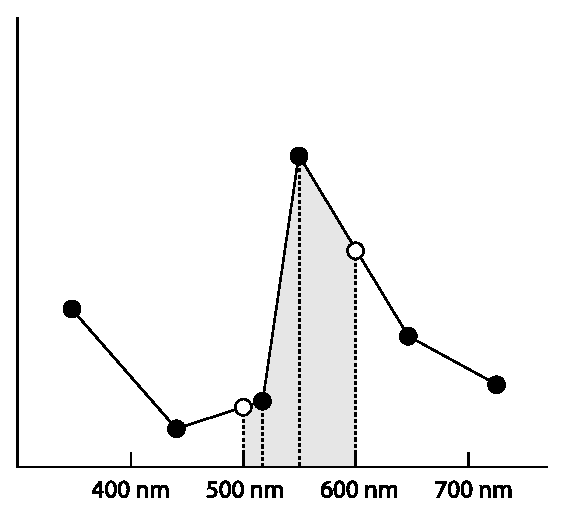
\includegraphics[width=0.4\linewidth]{chap05/IrregularSPDresample.eps}
    \caption{当重采样不规则定义的SPD时,我们需要计算由SPD样本定义的
        分段线性函数的均值。这里,我们想求从500nm到600nm的均值——图像下的阴影区。
        函数\refvar{AverageSpectrumSamples}{()}通过计算该图中虚线表示的每个区域的面积来完成。}
    \label{fig:5.2}
\end{figure}

\begin{lstlisting}
`\initcode{Spectrum Method Definitions}{=}\initnext{SpectrumMethodDefinitions}`
`\refvar{Float}{}` `\initvar{AverageSpectrumSamples}{}`(const `\refvar{Float}{}` *lambda, const `\refvar{Float}{}` *vals,
        int n, `\refvar{Float}{}` lambdaStart, `\refvar{Float}{}` lambdaEnd) {
    `\refcode{Handle cases with out-of-bounds range or single sample only}{}`
    `\refvar{Float}{}` sum = 0;
    `\refcode{Add contributions of constant segments before/after samples}{}`
    `\refcode{Advance to first relevant wavelength segment}{}`
    `\refcode{Loop over wavelength sample segments and add contributions}{}`
    return sum / (lambdaEnd - lambdaStart);
}
\end{lstlisting}

该函数从检查和处理极端情况开始,即求均值的波长范围
超出了提供的波长范围或只有单个样本进而均值计算是平凡的情况。
我们假设SPD在超出提供的采样范围外有常值(在两个端点的值);
如果这对于特定数据集不是一个合理的假设,则提供的数据应该在端点处有显式值(例如)0。
\begin{lstlisting}
`\initcode{Handle cases with out-of-bounds range or single sample only}{=}`
if (lambdaEnd   <= lambda[0])     return vals[0];
if (lambdaStart >= lambda[n - 1]) return vals[n - 1];
if (n == 1) return vals[0];
\end{lstlisting}

处理了这些情况后,下一步是检查看求均值的范围是否有部分超出第一个和/或最后一个样本值。
如果是,则我们累积常数段的贡献,用超出边界的波长范围缩放它。
\begin{lstlisting}
`\initcode{Add contributions of constant segments before/after samples}{=}`
if (lambdaStart < lambda[0])
    sum += vals[0] * (lambda[0] - lambdaStart);
if (lambdaEnd > lambda[n-1])
    sum += vals[n - 1] * (lambdaEnd - lambda[n - 1]);
\end{lstlisting}

现在我们推进到首个索引{\ttfamily i},
插值范围的起始波长重合于从$\lambda_i$到$\lambda_{i+1}$的一段。
这里更高效的实现是用二叉搜索而不是线性搜索
\footnote{甚至更高效的实现是利用一个事实即调用代码一般会需要
    在一段相邻波长范围上插值后的值,并可能在单次调用中接收了全部范围。
    然后可以为下一次插值从上一结尾处开始逐步寻找起始索引。}。
然而,该代码目前只在场景初始化时调用,所以目前不优化它不会影响渲染性能。
\begin{lstlisting}
`\initcode{Advance to first relevant wavelength segment}{=}`
int i = 0;
while (lambdaStart > lambda[i + 1]) ++i;
\end{lstlisting}

下面的循环在与求均值的范围重合的每个线性段上迭代。
对于每一段,它都通过求函数在这两点上取值的均值来
计算在波长范围{\ttfamily segLambdaStart}到{\ttfamily segLambdaEnd}上的均值。
该值依次用{\ttfamily interp()}计算,它是在给定波长的两个端点间线性插值的匿名函数。

下面调用{\ttfamily std::min()}和{\ttfamily std::max()}计算波长范围以在该段内做平均;
注意它们自然处理了{\ttfamily lambdaStart}、{\ttfamily lambdaEnd}或两者都在当前段内的情况。
\begin{lstlisting}
`\initcode{Loop over wavelength sample segments and add contributions}{=}`
auto interp = [lambda, vals](`\refvar{Float}{}` w, int i) {
    return `\refvar{Lerp}{}`((w - lambda[i]) / (lambda[i + 1] - lambda[i]),
                vals[i], vals[i + 1]);
};
for (; i+1 < n && lambdaEnd >= lambda[i]; ++i) {
    `\refvar{Float}{}` segLambdaStart = std::max(lambdaStart, lambda[i]);
    `\refvar{Float}{}` segLambdaEnd =   std::min(lambdaEnd,   lambda[i + 1]);
    sum += 0.5 * (interp(segLambdaStart, i) + interp(segLambdaEnd, i)) *
        (segLambdaEnd - segLambdaStart);
}
\end{lstlisting}

\subsection{XYZ颜色}\label{sub:XYZ颜色}
人类视觉系统的一个非凡性质是可只用三个浮点数为人类感知表示颜色。
颜色感知的\keyindex{三刺激理论}{tristimulus theory}{}说
用三个值$x_{\lambda},y_{\lambda}$和$z_{\lambda}$就能为人类观察者准确表示所有可见SPD。
给定发射SPD即$S(\lambda)$,通过积分它们与\keyindex{光谱匹配曲线}{spectral matching curve}{}
$X(\lambda),Y(\lambda)$和$Z(\lambda)$的积可算得这些值:
\begin{align}\label{eq:5.1}
    x_{\lambda} & =\int\limits_{\lambda}{S(\lambda)X(\lambda)\mathrm{d}\lambda}\, ,\nonumber \\
    y_{\lambda} & =\int\limits_{\lambda}{S(\lambda)Y(\lambda)\mathrm{d}\lambda}\, ,          \\
    z_{\lambda} & =\int\limits_{\lambda}{S(\lambda)Z(\lambda)\mathrm{d}\lambda}\, .\nonumber
\end{align}

这些曲线是由国际照明委员会\sidenote{译者注:法文Commission Internationale de l'Éclairage,
    英文International Commission on Illumination,是有关光学、照明、颜色和色度空间科学领域的国际组织,成立于1913年。}(CIE)
规范化机构在一系列以人类为测试对象的实验后决定的并画于\reffig{5.3}中。
一般认为这些匹配曲线通常类似于人类视网膜中三种色敏视锥细胞\sidenote{译者注:原文 color-sensitive cone。}的响应。
惊人的是,有截然不同分布的SPD可能有非常接近的$x_{\lambda},y_{\lambda}$和$z_{\lambda}$值。
对于人类观察者,这样的SPD实际上有一样的视觉呈现。
这样的光谱对称为\keyindex{同色异谱}{metamer}{}。
\begin{figure}[htbp]
    \centering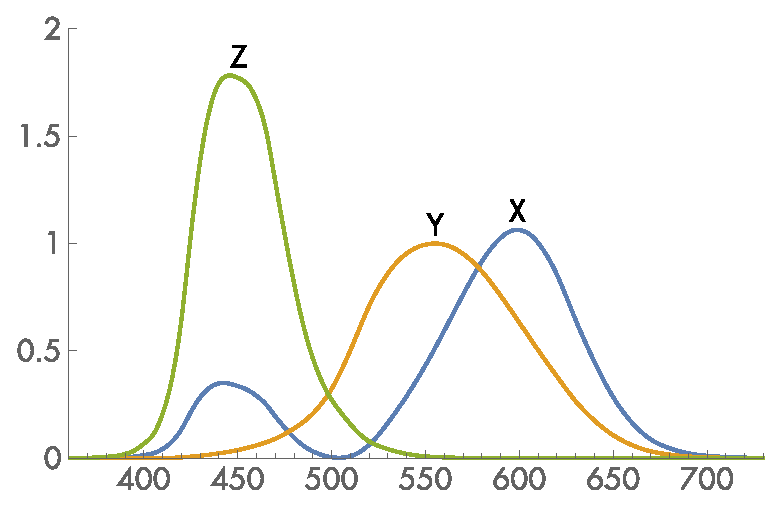
\includegraphics[width=0.5\linewidth]{chap05/matching-xyz.eps}
    \caption{对任意SPD计算XYZ值。用\refeq{5.1}让SPD与三个匹配曲线的每一个
    相乘并在其非零范围上积分以计算$x_{\lambda},y_{\lambda}$和$z_{\lambda}$值。}
    \label{fig:5.3}
\end{figure}

这给我们带来了关于光谱功率分布表示的一个微妙之处。
大部分颜色空间都希望模型颜色是对人类可见的,进而根据颜色感知的三刺激理论只需用三个系数。
尽管XYZ能很好地表示要对人类观察者显示的给定SPD,
但它对于光谱计算而言{\itshape 不是}特别好的基函数集。
例如,尽管XYZ值能很好地分别描述柠檬皮或荧光灯的感知颜色(回想\reffig{5.1}),
但它们各自的XYZ值之积给出的XYZ颜色可能明显不同于用其SPD更精确的表示相乘再计算出的XYZ值。

pbrt提供了标准$X(\lambda),Y(\lambda)$和$Z(\lambda)$相应曲线从360nm到830nm间隔1nm采样的值。
下面的数组中第$i$个样本的波长由\refvar{CIE\_lambda}{}的第$i$个元素给定;
用这种方式显式表示样本波长能更容易将XYZ样本传入到像\refvar{AverageSpectrumSamples}{()}
那样接收波长数组作为参数的函数。
\begin{lstlisting}
`\initcode{Spectral Data Declarations}{=}\initnext{SpectralDataDeclarations}`
static const int `\initvar{nCIESamples}{}` = 471;
extern const `\refvar{Float}{}` `\initvar{CIE\_X}{}`[`\refvar{nCIESamples}{}`];
extern const `\refvar{Float}{}` `\initvar{CIE\_Y}{}`[`\refvar{nCIESamples}{}`];
extern const `\refvar{Float}{}` `\initvar{CIE\_Z}{}`[`\refvar{nCIESamples}{}`];
extern const `\refvar{Float}{}` `\initvar{CIE\_lambda}{}`[`\refvar{nCIESamples}{}`];
\end{lstlisting}

\refvar{SampledSpectrum}{}用这些样本计算其光谱表示里的XYZ匹配曲线(即它们自己是\refvar{SampledSpectrum}{})。
\begin{lstlisting}
`\initcode{SampledSpectrum Private Data}{=}\initnext{SampledSpectrumPrivateData}`
static `\refvar{SampledSpectrum}{}` `\initvar[SampledSpectrum::X]{X}{}`, `\initvar[SampledSpectrum::Y]{Y}{}`, `\initvar[SampledSpectrum::Z]{Z}{}`;
\end{lstlisting}

\refvar{SampledSpectrum}{}的XYZ曲线在方法\refvar{SampledSpectrum::Init}{()}中算得,
它在系统启动时被定义于\refsec{初始化和渲染选项}\sidenote{译者注:原文标错了章节,已修正。}
的函数\refvar{pbrtInit}{()}调用。
\begin{lstlisting}
`\refcode{SampledSpectrum Public Methods}{+=}\lastnext{SampledSpectrumPublicMethods}`
static void `\initvar[SampledSpectrum::Init]{Init}{}`() {
    `\refcode{Compute XYZ matching functions for SampledSpectrum}{}`
    `\refcode{Compute RGB to spectrum functions for SampledSpectrum}{}`
}
\end{lstlisting}
\begin{lstlisting}
`\initcode{General pbrt Initialization}{=}`
`\refvar{SampledSpectrum}{}`::`\refvar[SampledSpectrum::Init]{Init}{}`();
\end{lstlisting}

为\refvar{SampledSpectrum}{}给定波长范围和样本数量,
为每个样本计算匹配函数的值只需计算样本的波长范围并利用\refvar{AverageSpectrumSamples}{()}例程。
\begin{lstlisting}
`\initcode{Compute XYZ matching functions for SampledSpectrum}{=}`
for (int i = 0; i < `\refvar{nSpectralSamples}{}`; ++i) {
    `\refvar{Float}{}` wl0 = `\refvar{Lerp}{}`(`\refvar{Float}{}`(i) / `\refvar{Float}{}`(`\refvar{nSpectralSamples}{}`), 
                     `\refvar{sampledLambdaStart}{}`, `\refvar{sampledLambdaEnd}{}`);
    `\refvar{Float}{}` wl1 = `\refvar{Lerp}{}`(`\refvar{Float}{}`(i + 1) / `\refvar{Float}{}`(`\refvar{nSpectralSamples}{}`), 
                     `\refvar{sampledLambdaStart}{}`, `\refvar{sampledLambdaEnd}{}`);
    `\refvar[SampledSpectrum::X]{X}{}`.`\refvar[CoefficientSpectrum::c]{c}{}`[i] = `\refvar{AverageSpectrumSamples}{}`(`\refvar{CIE\_lambda}{}`, `\refvar{CIE\_X}{}`, `\refvar{nCIESamples}{}`,
                                    wl0, wl1);
    `\refvar[SampledSpectrum::Y]{Y}{}`.`\refvar[CoefficientSpectrum::c]{c}{}`[i] = `\refvar{AverageSpectrumSamples}{}`(`\refvar{CIE\_lambda}{}`, `\refvar{CIE\_Y}{}`, `\refvar{nCIESamples}{}`,
                                    wl0, wl1);
    `\refvar[SampledSpectrum::Z]{Z}{}`.`\refvar[CoefficientSpectrum::c]{c}{}`[i] = `\refvar{AverageSpectrumSamples}{}`(`\refvar{CIE\_lambda}{}`, `\refvar{CIE\_Z}{}`, `\refvar{nCIESamples}{}`,
                                    wl0, wl1);
}
\end{lstlisting}

pbrt中所有\refvar{Spectrum}{}实现都必须提供将其SPD转换为$(x_{\lambda},y_{\lambda},z_{\lambda})$系数的方法。
例如,在更新图像像素的过程中就会调用该方法。
当\refvar{Spectrum}{}表示的沿相机射出的光线上的光提供给\refvar{Film}{}时,
\refvar{Film}{}最终将它们转换为用于存储和/或显示的RGB值时处理的第一步就是将SPD转换为XYZ系数。

为了计算XYZ系数,\refvar{SampledSpectrum}{}用黎曼和计算\refeq{5.1}的积分:
\begin{align*}
    x_{\lambda}\approx\frac{\lambda_{\text{end}}-\lambda_{\text{start}}}{N}\sum\limits_{i=0}^{N-1}{X_ic_i}\, ,
\end{align*}
并以此类推\sidenote{译者注:但是下面的代码中实际上还多除以了{\ttfamily CIE\_Y\_integral}。}。
\begin{lstlisting}
`\refcode{SampledSpectrum Public Methods}{+=}\lastnext{SampledSpectrumPublicMethods}`
void `\initvar{ToXYZ}{}`(`\refvar{Float}{}` xyz[3]) const {
    xyz[0] = xyz[1] = xyz[2] = 0.f;
    for (int i = 0; i < `\refvar{nSpectralSamples}{}`; ++i) {
        xyz[0] += `\refvar[SampledSpectrum::X]{X}{}`.`\refvar[CoefficientSpectrum::c]{c}{}`[i] * `\refvar[CoefficientSpectrum::c]{c}{}`[i];
        xyz[1] += `\refvar[SampledSpectrum::Y]{Y}{}`.`\refvar[CoefficientSpectrum::c]{c}{}`[i] * `\refvar[CoefficientSpectrum::c]{c}{}`[i];
        xyz[2] += `\refvar[SampledSpectrum::Z]{Z}{}`.`\refvar[CoefficientSpectrum::c]{c}{}`[i] * `\refvar[CoefficientSpectrum::c]{c}{}`[i];
    }
    `\refvar{Float}{}` scale = `\refvar{Float}{}`(`\refvar{sampledLambdaEnd}{}` - `\refvar{sampledLambdaStart}{}`) /
                  `\refvar{Float}{}`(CIE_Y_integral * `\refvar{nSpectralSamples}{}`);
    xyz[0] *= scale;
    xyz[1] *= scale;
    xyz[2] *= scale;
}
\end{lstlisting}

XYZ颜色的$y$系数与\keyindex{光亮度}{luminance}{}密切相关,
它度量颜色的感知亮度\sidenote{译者注:原文brightness。}。
亮度将在\refsub{光亮度与光度学}详细介绍。
我们提供了分开的方法单独计算$y$,因为经常只需要光谱的亮度
(例如第\refchap{光传输I:表面反射}、\refchap{光传输II:体积渲染}和\refchap{光传输III:双向方法}中的
一些光传输算法用亮度作为穿过场景的光路的相对重要性度量)。
\begin{lstlisting}
`\refcode{SampledSpectrum Public Methods}{+=}\lastnext{SampledSpectrumPublicMethods}`
`\refvar{Float}{}` `\initvar[SampledSpectrum::y]{y}{}`() const { 
    `\refvar{Float}{}` yy = 0.f;
    for (int i = 0; i < `\refvar{nSpectralSamples}{}`; ++i)
        yy += `\refvar[SampledSpectrum::Y]{Y}{}`.`\refvar[CoefficientSpectrum::c]{c}{}`[i] * `\refvar[CoefficientSpectrum::c]{c}{}`[i];
    return yy * `\refvar{Float}{}`(`\refvar{sampledLambdaEnd}{}` - `\refvar{sampledLambdaStart}{}`) /
        `\refvar{Float}{}`(`\refvar{nSpectralSamples}{}`);
}
\end{lstlisting}

\subsection{RGB颜色}\label{sub:RGB颜色}

当我们在显示器上显示RGB颜色时,实际展示的光谱基本上决定于三种光谱响应曲线的加权和,
红、绿、蓝各一种,由显示器的磷光体\sidenote{译者注:原文phosphor。}发出,例如LED
\sidenote{译者注:即light-emitting diode,发光二极管。}
或LCD\sidenote{译者注:即liquid-crystal display,液晶显示器。}元素,
或者等离子体胞\sidenote{译者注:原文plasma cell。}
\footnote{该模型确实作了简化,它忽略了显示器所作的任何额外处理;
    尤其是许多显示器对显示的值执行了非线性重映射。}。
\reffig{5.4}画出了LED显示器和LCD显示器发出的红、绿和蓝分布;
注意它们截然不同。
\begin{figure}[htbp]
    \centering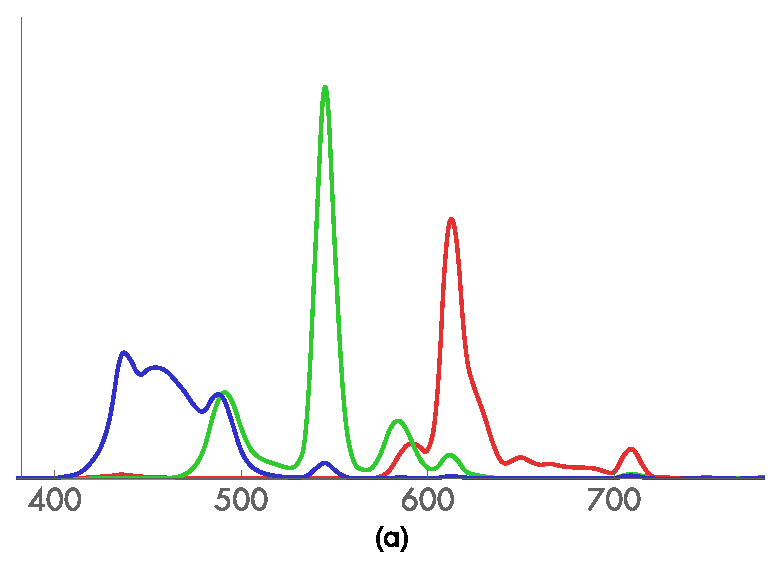
\includegraphics[width=0.45\linewidth]{chap05/lcd-display-spd.eps}\,
    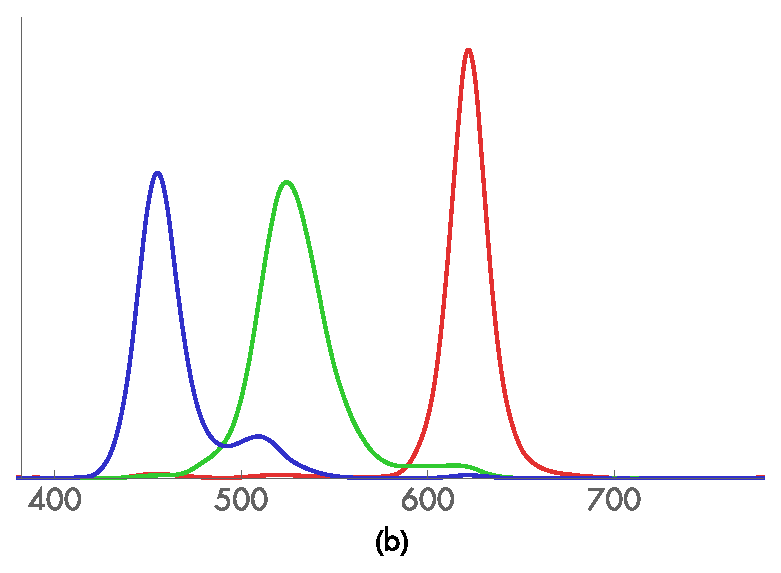
\includegraphics[width=0.45\linewidth]{chap05/led-display-spd.eps}
    \caption{LCD显示器和LED显示器的红、绿和蓝发射曲线。
    第一幅图展示了LCD显示器的曲线,第二幅图展示了LED的。
    这两种显示器有完全不同的发射配置({\itshape 感谢X-Rite公司提供数据})。}
    \label{fig:5.4}
\end{figure}

\reffig{5.5}依次展示了在这些显示器上显示RGB颜色$(0.6,0.3,0.2)$的SPD结果。
不出意料,结果中SPD也截然不同。这个例子说明了当用户选择RGB值时,
用他们提供的RGB值来描述特定颜色实际上只有在给定他们所用的显示器特性知识时才有意义。
\begin{figure}[htbp]
    \centering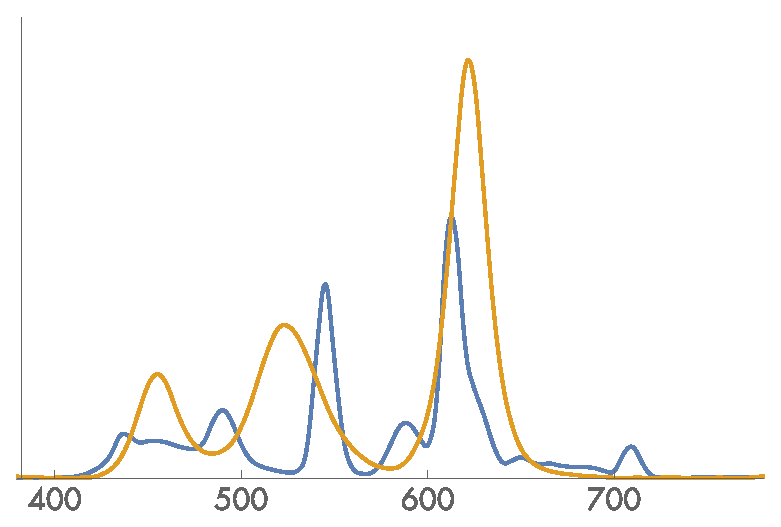
\includegraphics[width=0.5\linewidth]{chap05/same-rgb-different-display.eps}
    \caption{在LED和LCD显示器上显示RGB颜色$(0.6,0.3,0.2)$的SPD。
        甚至给定相同RGB值时得到的发射SPD也明显不同,因为\reffig{5.4}中的发射曲线不同。}
    \label{fig:5.5}
\end{figure}

给定SPD的表示$(x_{\lambda},y_{\lambda},z_{\lambda})$,
为感兴趣的显示器选定好定义红、绿和蓝的特定SPD集后,
我们可以将其转换为相应的RGB系数。
对于特定显示器,有了光谱响应曲线$R(\lambda),G(\lambda)$和$B(\lambda)$后,
可以通过积分响应曲线和SPD即$S(\lambda)$以及利用颜色感知的三刺激理论算得RGB系数:
\begin{align*}
    r & =\int R(\lambda)S(\lambda)\mathrm{d}\lambda=\int R(\lambda)(x_{\lambda}X(\lambda)+y_{\lambda}Y(\lambda)+z_{\lambda}Z(\lambda))\mathrm{d}\lambda                        \\
      & =x_{\lambda}\int R(\lambda)X(\lambda)\mathrm{d}\lambda+y_{\lambda}\int R(\lambda)Y(\lambda)\mathrm{d}\lambda+z_{\lambda}\int R(\lambda)Z(\lambda)\mathrm{d}\lambda\, .
\end{align*}

对于给定的响应曲线可以预先计算积$R(\lambda)X(\lambda)$的积分等,
使得能够把整个转换表达为矩阵:
\begin{align*}
    \left[\begin{array}{c}
            r \\ g\\ b
        \end{array}\right]=\left[
        \begin{array}{ccc}
            \int R(\lambda)X(\lambda)\mathrm{d}\lambda & \int R(\lambda)Y(\lambda)\mathrm{d}\lambda & \int R(\lambda)Z(\lambda)\mathrm{d}\lambda \\
            \int G(\lambda)X(\lambda)\mathrm{d}\lambda & \int G(\lambda)Y(\lambda)\mathrm{d}\lambda & \int G(\lambda)Z(\lambda)\mathrm{d}\lambda \\
            \int B(\lambda)X(\lambda)\mathrm{d}\lambda & \int B(\lambda)Y(\lambda)\mathrm{d}\lambda & \int B(\lambda)Z(\lambda)\mathrm{d}\lambda
        \end{array}
        \right]\left[\begin{array}{c}
            x_{\lambda} \\ y_{\lambda} \\ z_{\lambda}
        \end{array}\right]\, .
\end{align*}

pbrt中实现的转换例程是基于为高清电视定义的RGB光谱标准集的
\sidenote{译者注:这些系数的来由可见译者补充的\refsub{色度学}。}。
\begin{lstlisting}
`\refcode{Spectrum Utility Declarations}{+=}\lastnext{SpectrumUtilityDeclarations}`
inline void `\initvar{XYZToRGB}{}`(const `\refvar{Float}{}` xyz[3], `\refvar{Float}{}` rgb[3]) {
    rgb[0] =  3.240479f*xyz[0] - 1.537150f*xyz[1] - 0.498535f*xyz[2];
    rgb[1] = -0.969256f*xyz[0] + 1.875991f*xyz[1] + 0.041556f*xyz[2];
    rgb[2] =  0.055648f*xyz[0] - 0.204043f*xyz[1] + 1.057311f*xyz[2];
}
\end{lstlisting}

该矩阵的逆给出了把以特定RGB响应曲线表达的给定RGB值转换为$(x_{\lambda},y_{\lambda},z_{\lambda})$系数的系数。
\begin{lstlisting}
`\refcode{Spectrum Utility Declarations}{+=}\lastnext{SpectrumUtilityDeclarations}`
inline void `\initvar{RGBToXYZ}{}`(const `\refvar{Float}{}` rgb[3], `\refvar{Float}{}` xyz[3]) {
    xyz[0] = 0.412453f*rgb[0] + 0.357580f*rgb[1] + 0.180423f*rgb[2];
    xyz[1] = 0.212671f*rgb[0] + 0.715160f*rgb[1] + 0.072169f*rgb[2];
    xyz[2] = 0.019334f*rgb[0] + 0.119193f*rgb[1] + 0.950227f*rgb[2];
}
\end{lstlisting}

有了这些函数,\refvar{SampledSpectrum}{}可以通过首先转换到XYZ
再用实用函数\refvar{XYZToRGB}{()}转换为RGB系数。
\begin{lstlisting}
`\refcode{SampledSpectrum Public Methods}{+=}\lastnext{SampledSpectrumPublicMethods}`
void `\initvar[SampledSpectrum::ToRGB]{ToRGB}{}`(`\refvar{Float}{}` rgb[3]) const { 
    `\refvar{Float}{}` xyz[3];
    `\refvar{ToXYZ}{}`(xyz);
    `\refvar{XYZToRGB}{}`(xyz, rgb);
}
\end{lstlisting}

用方法\refvar[SampledSpectrum::ToRGBSpectrum]{ToRGBSpectrum}{()}也能很容易地创建\refvar{RGBSpectrum}{}。
\begin{lstlisting}
`\refcode{SampledSpectrum Public Methods}{+=}\lastnext{SampledSpectrumPublicMethods}`
`\refvar{RGBSpectrum}{}` `\initvar[SampledSpectrum::ToRGBSpectrum]{ToRGBSpectrum}{}`() const;
\end{lstlisting}

反过来从RGB或XYZ值转换为SPD并不简单:问题是高度欠约束的。
回想无数个不同的SPD有相同的$(x_{\lambda},y_{\lambda},z_{\lambda})$(进而以及RGB)系数。
因此,给定RGB或$(x_{\lambda},y_{\lambda},z_{\lambda})$值,可为其选择无数种可能的SPD。
有许多我们希望转换函数具有的准则:
\begin{itemize}
    \item 如果所有RGB系数有相同的值,则结果SPD应该为常数。
    \item 一般而言,希望算出的SPD是光滑的。大多数真实世界物体都有相对光滑的光谱。
          (尖锐光谱的主要源头是光源,特别是荧光灯。幸运的是,对于光源实际的光谱数据比反射率更常见。)
\end{itemize}

光滑目标是为什么把SPD构建为显示器的$R(\lambda),G(\lambda)$和$B(\lambda)$SPD的加权和不是好办法的原因:
如\reffig{5.4}所示,这些函数一般都是不规则且尖锐的,
因此它们的加权和不会是非常光滑的SPD。
该结果和给定RGB值是同色异谱的,它不太可能是实际物体SPD的准确表示。

这里我们实现了\citet{10.1080/10867651.1999.10487511}提出的将RGB转换为SPD
并尝试实现以上目标的的方法。
该方法基于一点观察即最好从为红、绿和蓝计算单独的光滑SPD开始,
这样用给定RGB系数计算它们的加权和然后转换回RGB给出的结果会接近于原来的RGB系数。
他通过数值优化过程发现了这样的光谱。

\citeauthor{10.1080/10867651.1999.10487511}观察到
可以对该方法做额外两点提升。
第一,比起用算得的恰好不是常数的红、绿和蓝SPD之和来表示常数光谱,
用常数SPD表示常数光谱更好。
第二,像黄色(红绿混合)那样由两种原色混合的颜色,
用它们预先计算的光滑SPD表示比用两种相应原色的SPD之和表示更好。

下面的数组保存了符合这些准则的SPD,
其样本的波长在\refvar{RGB2SpectLambda}{[]}
中(这些数据由Karl vom Berge生成)
\sidenote{译者注:cyan指蓝绿色,也称青色,magenta指紫红色,也称品红、洋红。}。
\begin{lstlisting}
`\refcode{Spectral Data Declarations}{+=}\lastnext{SpectralDataDeclarations}`
static const int `\initvar{nRGB2SpectSamples}{}` = 32;
extern const `\refvar{Float}{}` `\initvar{RGB2SpectLambda}{}`[`\refvar{nRGB2SpectSamples}{}`];
extern const `\refvar{Float}{}` `\initvar{RGBRefl2SpectWhite}{}`[`\refvar{nRGB2SpectSamples}{}`];
extern const `\refvar{Float}{}` `\initvar{RGBRefl2SpectCyan}{}`[`\refvar{nRGB2SpectSamples}{}`];
extern const `\refvar{Float}{}` `\initvar{RGBRefl2SpectMagenta}{}`[`\refvar{nRGB2SpectSamples}{}`];
extern const `\refvar{Float}{}` `\initvar{RGBRefl2SpectYellow}{}`[`\refvar{nRGB2SpectSamples}{}`];
extern const `\refvar{Float}{}` `\initvar{RGBRefl2SpectRed}{}`[`\refvar{nRGB2SpectSamples}{}`];
extern const `\refvar{Float}{}` `\initvar{RGBRefl2SpectGreen}{}`[`\refvar{nRGB2SpectSamples}{}`];
extern const `\refvar{Float}{}` `\initvar{RGBRefl2SpectBlue}{}`[`\refvar{nRGB2SpectSamples}{}`];
\end{lstlisting}

如果给定的RGB颜色为光源描述了光照,则用典型光源的光谱功率分布
计算用于反射率的转换表以定义“白色”会比用常数光谱得到更好结果。
数组\refvar{RGBIllum2Spect}{}使用了D65光谱功率分布,
它被CIE标准化为表示正午日光(\refsub{标准光源}将更多讨论D65光源)。
\begin{lstlisting}
`\refcode{Spectral Data Declarations}{+=}\lastcode{SpectralDataDeclarations}`
extern const `\refvar{Float}{}` `\initvar{RGBIllum2SpectWhite}{}`[`\refvar{nRGB2SpectSamples}{}`];
extern const `\refvar{Float}{}` `\initvar{RGBIllum2SpectCyan}{}`[`\refvar{nRGB2SpectSamples}{}`];
extern const `\refvar{Float}{}` `\initvar{RGBIllum2SpectMagenta}{}`[`\refvar{nRGB2SpectSamples}{}`];
extern const `\refvar{Float}{}` `\initvar{RGBIllum2SpectYellow}{}`[`\refvar{nRGB2SpectSamples}{}`];
extern const `\refvar{Float}{}` `\initvar{RGBIllum2SpectRed}{}`[`\refvar{nRGB2SpectSamples}{}`];
extern const `\refvar{Float}{}` `\initvar{RGBIllum2SpectGreen}{}`[`\refvar{nRGB2SpectSamples}{}`];
extern const `\refvar{Float}{}` `\initvar{RGBIllum2SpectBlue}{}`[`\refvar{nRGB2SpectSamples}{}`];
\end{lstlisting}

代码片\refcode{Compute RGB to spectrum functions for SampledSpectrum}{}由\linebreak
\refvar{SampledSpectrum::Init}{()}调用,此处不再介绍\sidenote{译者注:我补充回来了。};
它通过用函数\linebreak\refvar{AverageSpectrumSamples}{()}重采样
分布{\ttfamily RGBRefl2Spect}和{\ttfamily RGBIllum2Spect}来
初始化下列的\refvar{SampledSpectrum}{}值。
\begin{lstlisting}
`\refcode{SampledSpectrum Private Data}{+=}\lastnext{SampledSpectrumPrivateData}`
static `\refvar{SampledSpectrum}{}` `\initvar{rgbRefl2SpectWhite}{}`, `\initvar{rgbRefl2SpectCyan}{}`;
static `\refvar{SampledSpectrum}{}` `\initvar{rgbRefl2SpectMagenta}{}`, `\initvar{rgbRefl2SpectYellow}{}`;
static `\refvar{SampledSpectrum}{}` `\initvar{rgbRefl2SpectRed}{}`, `\initvar{rgbRefl2SpectGreen}{}`;
static `\refvar{SampledSpectrum}{}` `\initvar{rgbRefl2SpectBlue}{}`;
\end{lstlisting}
\begin{lstlisting}
`\refcode{SampledSpectrum Private Data}{+=}\lastcode{SampledSpectrumPrivateData}`
static `\refvar{SampledSpectrum}{}` `\initvar{rgbIllum2SpectWhite}{}`, `\initvar{rgbIllum2SpectCyan}{}`;
static `\refvar{SampledSpectrum}{}` `\initvar{rgbIllum2SpectMagenta}{}`, `\initvar{rgbIllum2SpectYellow}{}`;
static `\refvar{SampledSpectrum}{}` `\initvar{rgbIllum2SpectRed}{}`, `\initvar{rgbIllum2SpectGreen}{}`;
static `\refvar{SampledSpectrum}{}` `\initvar{rgbIllum2SpectBlue}{}`;
\end{lstlisting}
\begin{lstlisting}
`\initcode{Compute RGB to spectrum functions for SampledSpectrum}{=}`
for (int i = 0; i < `\refvar{nSpectralSamples}{}`; ++i) {
    `\refvar{Float}{}` wl0 = `\refvar{Lerp}{}`(`\refvar{Float}{}`(i) / `\refvar{Float}{}`(`\refvar{nSpectralSamples}{}`), 
                     `\refvar{sampledLambdaStart}{}`, `\refvar{sampledLambdaEnd}{}`);
    `\refvar{Float}{}` wl1 = `\refvar{Lerp}{}`(`\refvar{Float}{}`(i+1) / `\refvar{Float}{}`(`\refvar{nSpectralSamples}{}`), 
                     `\refvar{sampledLambdaStart}{}`, `\refvar{sampledLambdaEnd}{}`);
    `\refvar{rgbRefl2SpectWhite}{}`.`\refvar[CoefficientSpectrum::c]{c}{}`[i] = `\refvar{AverageSpectrumSamples}{}`(`\refvar{RGB2SpectLambda}{}`, `\refvar{rgbRefl2SpectWhite}{}`, 
        `\refvar{nRGB2SpectSamples}{}`, wl0, wl1);
    `\refvar{rgbRefl2SpectCyan}{}`.`\refvar[CoefficientSpectrum::c]{c}{}`[i] = `\refvar{AverageSpectrumSamples}{}`(`\refvar{RGB2SpectLambda}{}`, `\refvar{rgbRefl2SpectCyan}{}`, 
        `\refvar{nRGB2SpectSamples}{}`, wl0, wl1);
    `\refvar{rgbRefl2SpectMagenta}{}`.`\refvar[CoefficientSpectrum::c]{c}{}`[i] = `\refvar{AverageSpectrumSamples}{}`(`\refvar{RGB2SpectLambda}{}`, `\refvar{rgbRefl2SpectMagenta}{}`, 
        `\refvar{nRGB2SpectSamples}{}`, wl0, wl1);
    `\refvar{rgbRefl2SpectYellow}{}`.`\refvar[CoefficientSpectrum::c]{c}{}`[i] = `\refvar{AverageSpectrumSamples}{}`(`\refvar{RGB2SpectLambda}{}`, `\refvar{rgbRefl2SpectYellow}{}`, 
        `\refvar{nRGB2SpectSamples}{}`, wl0, wl1);
    `\refvar{rgbRefl2SpectRed}{}`.`\refvar[CoefficientSpectrum::c]{c}{}`[i] = `\refvar{AverageSpectrumSamples}{}`(`\refvar{RGB2SpectLambda}{}`, `\refvar{rgbRefl2SpectRed}{}`, 
        `\refvar{nRGB2SpectSamples}{}`, wl0, wl1);
    `\refvar{rgbRefl2SpectGreen}{}`.`\refvar[CoefficientSpectrum::c]{c}{}`[i] = `\refvar{AverageSpectrumSamples}{}`(`\refvar{RGB2SpectLambda}{}`, `\refvar{rgbRefl2SpectGreen}{}`, 
        `\refvar{nRGB2SpectSamples}{}`, wl0, wl1);
    `\refvar{rgbRefl2SpectBlue}{}`.`\refvar[CoefficientSpectrum::c]{c}{}`[i] = `\refvar{AverageSpectrumSamples}{}`(`\refvar{RGB2SpectLambda}{}`, `\refvar{rgbRefl2SpectBlue}{}`, 
        `\refvar{nRGB2SpectSamples}{}`, wl0, wl1);

    `\refvar{rgbIllum2SpectWhite}{}`.`\refvar[CoefficientSpectrum::c]{c}{}`[i] = `\refvar{AverageSpectrumSamples}{}`(`\refvar{RGB2SpectLambda}{}`, `\refvar{rgbIllum2SpectWhite}{}`, 
        `\refvar{nRGB2SpectSamples}{}`, wl0, wl1);
    `\refvar{rgbIllum2SpectCyan}{}`.`\refvar[CoefficientSpectrum::c]{c}{}`[i] = `\refvar{AverageSpectrumSamples}{}`(`\refvar{RGB2SpectLambda}{}`, `\refvar{rgbIllum2SpectCyan}{}`, 
        `\refvar{nRGB2SpectSamples}{}`, wl0, wl1);
    `\refvar{rgbIllum2SpectMagenta}{}`.`\refvar[CoefficientSpectrum::c]{c}{}`[i] = `\refvar{AverageSpectrumSamples}{}`(`\refvar{RGB2SpectLambda}{}`, `\refvar{rgbIllum2SpectMagenta}{}`, 
        `\refvar{nRGB2SpectSamples}{}`, wl0, wl1);
    `\refvar{rgbIllum2SpectYellow}{}`.`\refvar[CoefficientSpectrum::c]{c}{}`[i] = `\refvar{AverageSpectrumSamples}{}`(`\refvar{RGB2SpectLambda}{}`, `\refvar{rgbIllum2SpectYellow}{}`, 
        `\refvar{nRGB2SpectSamples}{}`, wl0, wl1);
    `\refvar{rgbIllum2SpectRed}{}`.`\refvar[CoefficientSpectrum::c]{c}{}`[i] = `\refvar{AverageSpectrumSamples}{}`(`\refvar{RGB2SpectLambda}{}`, `\refvar{rgbIllum2SpectRed}{}`, 
        `\refvar{nRGB2SpectSamples}{}`, wl0, wl1);
    `\refvar{rgbIllum2SpectGreen}{}`.`\refvar[CoefficientSpectrum::c]{c}{}`[i] = `\refvar{AverageSpectrumSamples}{}`(`\refvar{RGB2SpectLambda}{}`, `\refvar{rgbIllum2SpectGreen}{}`, 
        `\refvar{nRGB2SpectSamples}{}`, wl0, wl1);
    `\refvar{rgbIllum2SpectBlue}{}`.`\refvar[CoefficientSpectrum::c]{c}{}`[i] = `\refvar{AverageSpectrumSamples}{}`(`\refvar{RGB2SpectLambda}{}`, `\refvar{rgbIllum2SpectBlue}{}`, 
        `\refvar{nRGB2SpectSamples}{}`, wl0, wl1);
}
\end{lstlisting}

方法\refvar{SampledSpectrum::FromRGB}{()}将给定RGB值转换为完整的SPD。
除了RGB值,它还接收一个指明RGB值是表示曲面反射率还是光源的枚举值;
相应的{\ttfamily rgbIllum2Spect}或{\ttfamily rgbRefl2Spect}值用于该转换。
\begin{lstlisting}
`\refcode{Spectrum Utility Declarations}{+=}\lastcode{SpectrumUtilityDeclarations}`
enum class `\initvar{SpectrumType}{}` { `\initvar{Reflectance}{}`, `\initvar{Illuminant}{}` };
\end{lstlisting}
\begin{lstlisting}
`\refcode{Spectrum Method Definitions}{+=}\lastnext{SpectrumMethodDefinitions}`
`\refvar{SampledSpectrum}{}` `\initvar{SampledSpectrum::FromRGB}{}`(const `\refvar{Float}{}` rgb[3],
                                         `\refvar{SpectrumType}{}` type) {
    `\refvar{SampledSpectrum}{}` r;
    if (type == `\refvar{SpectrumType}{}`::`\refvar{Reflectance}{}`) {
        `\refcode{Convert reflectance spectrum to RGB}{}`
    } else {
        `\refcode{Convert illuminant spectrum to RGB}{}`
    }
    return r.`\refvar[CoefficientSpectrum::Clamp]{Clamp}{}`();
}
\end{lstlisting}

这里我们将展示反射率的转换过程。光源的计算也类似,只是用的不同的转换系数
\sidenote{译者注:这里我补充了光源的代码。}。
首先,实现确定红、绿、蓝哪个通道最小。
\begin{lstlisting}
`\initcode{Convert reflectance spectrum to RGB}{=}`
if (rgb[0] <= rgb[1] && rgb[0] <= rgb[2]) {
    `\refcode{Compute reflectance SampledSpectrum with rgb[0] as minimum}{}`
} else if (rgb[1] <= rgb[0] && rgb[1] <= rgb[2]) {
    `\refcode{Compute reflectance SampledSpectrum with rgb[1] as minimum}{}`
} else {
    `\refcode{Compute reflectance SampledSpectrum with rgb[2] as minimum}{}`
}
\end{lstlisting}
\begin{lstlisting}
`\initcode{Convert illuminant spectrum to RGB}{=}` 
if (rgb[0] <= rgb[1] && rgb[0] <= rgb[2]) {
    `\refcode{Compute illuminant SampledSpectrum with rgb[0] as minimum}{}`
} else if (rgb[1] <= rgb[0] && rgb[1] <= rgb[2]) {
    `\refcode{Compute illuminant SampledSpectrum with rgb[1] as minimum}{}`
} else {
    `\refcode{Compute illuminant SampledSpectrum with rgb[2] as minimum}{}`
}
\end{lstlisting}

这里是红色分量最小情况下的代码(绿色和蓝色类似这里书中就不介绍了)
\sidenote{译者注:我补充回来了。}。
如果红色最小,则我们知道绿色和蓝色有比红色更大的值。
这样我们可以通过给其赋予红色分量值乘以\refvar{rgbRefl2SpectWhite}{}中的
白色光谱来开始转换最终要返回的SPD。
完成后,RGB值中剩下要处理的是$(0,g-r,b-r)$。
代码依次确定剩下两个分量谁最小。
该值乘以青色\sidenote{译者注:原文cyan。}(绿蓝)光谱并加到结果中,
我们还剩下$(0,g-b,0)$或$(0,0,b-g)$。
基于绿色或蓝色通道哪一个非零,绿色或蓝色通道SPD被剩余部分缩放完成转换。
\begin{lstlisting}
`\initcode{Compute reflectance SampledSpectrum with rgb[0] as minimum}{=}`
r += rgb[0] * `\refvar{rgbRefl2SpectWhite}{}`;
if (rgb[1] <= rgb[2]) {
    r += (rgb[1] - rgb[0]) * `\refvar{rgbRefl2SpectCyan}{}`;
    r += (rgb[2] - rgb[1]) * `\refvar{rgbRefl2SpectBlue}{}`;
} else {
    r += (rgb[2] - rgb[0]) * `\refvar{rgbRefl2SpectCyan}{}`;
    r += (rgb[1] - rgb[2]) * `\refvar{rgbRefl2SpectGreen}{}`;
}
\end{lstlisting}
\begin{lstlisting}
`\initcode{Compute reflectance SampledSpectrum with rgb[1] as minimum}{=}`
r += rgb[1] * `\refvar{rgbRefl2SpectWhite}{}`;
if (rgb[0] <= rgb[2]) {
    r += (rgb[0] - rgb[1]) * `\refvar{rgbRefl2SpectMagenta}{}`;
    r += (rgb[2] - rgb[0]) * `\refvar{rgbRefl2SpectBlue}{}`;
} else {
    r += (rgb[2] - rgb[1]) * `\refvar{rgbRefl2SpectMagenta}{}`;
    r += (rgb[0] - rgb[2]) * `\refvar{rgbRefl2SpectRed}{}`;
}
\end{lstlisting}
\begin{lstlisting}
`\initcode{Compute reflectance SampledSpectrum with rgb[2] as minimum}{=}`
r += rgb[2] * `\refvar{rgbRefl2SpectWhite}{}`;
if (rgb[0] <= rgb[1]) {
    r += (rgb[0] - rgb[2]) * `\refvar{rgbRefl2SpectYellow}{}`;
    r += (rgb[1] - rgb[0]) * `\refvar{rgbRefl2SpectGreen}{}`;
} else {
    r += (rgb[1] - rgb[2]) * `\refvar{rgbRefl2SpectYellow}{}`;
    r += (rgb[0] - rgb[1]) * `\refvar{rgbRefl2SpectRed}{}`;
}
\end{lstlisting}
\begin{lstlisting}
`\initcode{Compute illuminant SampledSpectrum with rgb[0] as minimum}{=}`
r += rgb[0] * `\refvar{rgbIllum2SpectWhite}{}`;
if (rgb[1] <= rgb[2]) {
    r += (rgb[1] - rgb[0]) * `\refvar{rgbIllum2SpectCyan}{}`;
    r += (rgb[2] - rgb[1]) * `\refvar{rgbIllum2SpectBlue}{}`;
} else {
    r += (rgb[2] - rgb[0]) * `\refvar{rgbIllum2SpectCyan}{}`;
    r += (rgb[1] - rgb[2]) * `\refvar{rgbIllum2SpectGreen}{}`;
}
\end{lstlisting}
\begin{lstlisting}
`\initcode{Compute illuminant SampledSpectrum with rgb[1] as minimum}{=}`
r += rgb[1] * `\refvar{rgbIllum2SpectWhite}{}`;
if (rgb[0] <= rgb[2]) {
    r += (rgb[0] - rgb[1]) * `\refvar{rgbIllum2SpectMagenta}{}`;
    r += (rgb[2] - rgb[0]) * `\refvar{rgbIllum2SpectBlue}{}`;
} else {
    r += (rgb[2] - rgb[1]) * `\refvar{rgbIllum2SpectMagenta}{}`;
    r += (rgb[0] - rgb[2]) * `\refvar{rgbIllum2SpectRed}{}`;
}
\end{lstlisting}
\begin{lstlisting}
`\initcode{Compute illuminant SampledSpectrum with rgb[2] as minimum}{=}`
r += rgb[2] * `\refvar{rgbIllum2SpectWhite}{}`;
if (rgb[0] <= rgb[1]) {
    r += (rgb[0] - rgb[2]) * `\refvar{rgbIllum2SpectYellow}{}`;
    r += (rgb[1] - rgb[0]) * `\refvar{rgbIllum2SpectGreen}{}`;
} else {
    r += (rgb[1] - rgb[2]) * `\refvar{rgbIllum2SpectYellow}{}`;
    r += (rgb[0] - rgb[1]) * `\refvar{rgbIllum2SpectRed}{}`;
}
\end{lstlisting}

有了从RGB转换的方法,从XYZ颜色转换也很容易。
我们首先从XYZ转换到RGB然后再用方法\refvar[SampledSpectrum::FromRGB]{FromRGB}{()}。
\begin{lstlisting}
`\refcode{SampledSpectrum Public Methods}{+=}\lastcode{SampledSpectrumPublicMethods}`
static `\refvar{SampledSpectrum}{}` `\initvar[SampledSpectrum::FromXYZ]{FromXYZ}{}`(const `\refvar{Float}{}` xyz[3],
        `\refvar{SpectrumType}{}` type = `\refvar{SpectrumType}{}`::`\refvar{Reflectance}{}`) {
    `\refvar{Float}{}` rgb[3];
    `\refvar{XYZToRGB}{}`(xyz, rgb);
    return `\refvar[SampledSpectrum::FromRGB]{FromRGB}{}`(rgb, type);
}
\end{lstlisting}

最后,我们再次用上述基础提供了转换类\refvar{RGBSpectrum}{}的实例的构造函数。
\begin{lstlisting}
`\refcode{Spectrum Method Definitions}{+=}\lastnext{SpectrumMethodDefinitions}`
`\refvar{SampledSpectrum}{}`::`\refvar{SampledSpectrum}{}`(const `\refvar{RGBSpectrum}{}` &r, `\refvar{SpectrumType}{}` t) {
    `\refvar{Float}{}` rgb[3];
    r.`\refvar[SampledSpectrum::ToRGB]{ToRGB}{}`(rgb);
    *this = `\refvar{SampledSpectrum}{}`::`\refvar[SampledSpectrum::FromRGB]{FromRGB}{}`(rgb, t);
}
\end{lstlisting}

\section{RGBSpectrum的实现}\label{sec:RGBSpectrum的实现}

这里\refvar{RGBSpectrum}{}的实现用红绿蓝分量的加权和表示SPD。
回想该表示是定义病态的:给定两个不同的计算机显示器,
让它们显示相同RGB值并不会让它们发射相同的SPD。
因此,为了给一组RGB值指定实际的SPD,我们必须知道定义时所依据的显示器原色;
这些信息一般不会随RGB值提供。

然而RGB表示很方便:几乎所有3D建模和设计工具都使用RGB颜色,
大多数3D内容都用RGB指定。
此外,它的计算和存储很高效,只需要三个浮点值表示。
我们的\refvar{RGBSpectrum}{}实现继承自\refvar{CoefficientSpectrum}{},
指定三个分量存储。
因此,之前定义的所有算术运算符都自动地适用于\refvar{RGBSpectrum}{}。
\begin{lstlisting}
`\refcode{Spectrum Declarations}{+=}\lastcode{SpectrumDeclarations}`
class `\initvar{RGBSpectrum}{}` : public `\refvar{CoefficientSpectrum}{}`<3> {
public:
    `\refcode{RGBSpectrum Public Methods}{}`
};
\end{lstlisting}
\begin{lstlisting}
`\initcode{RGBSpectrum Public Methods}{=}\initnext{RGBSpectrumPublicMethods}`
`\refvar{RGBSpectrum}{}`(`\refvar{Float}{}` v = 0.f) : `\refvar{CoefficientSpectrum}{}`<3>(v) { }
`\refvar{RGBSpectrum}{}`(const `\refvar{CoefficientSpectrum}{}`<3> &v) 
    : `\refvar{CoefficientSpectrum}{}`<3>(v) { }
\end{lstlisting}

除了基本算术运算,\refvar{RGBSpectrum}{}还需要提供方法来与XYZ和RGB表示互相转换。
这些对于\refvar{RGBSpectrum}{}是容易的。
注意\refvar[RGBSpectrum::FromRGB]{FromRGB}{()}接收像该方法的
\refvar{SampledSpectrum}{}实例那样的\refvar{SpectrumType}{}参数。
尽管这里没有使用,但这两个类的{\ttfamily FromRGB()}方法
必须有匹配的特征,这样系统剩下的部分可以一致地调用它们而不用管用的是哪种光谱表示。
\begin{lstlisting}
`\refcode{RGBSpectrum Public Methods}{+=}\lastnext{RGBSpectrumPublicMethods}`
static `\refvar{RGBSpectrum}{}` `\initvar[RGBSpectrum::FromRGB]{FromRGB}{}`(const `\refvar{Float}{}` rgb[3],
        `\refvar{SpectrumType}{}` type = `\refvar{SpectrumType}{}`::`\refvar{Reflectance}{}`) {
    `\refvar{RGBSpectrum}{}` s;
    s.`\refvar[CoefficientSpectrum::c]{c}{}`[0] = rgb[0];
    s.`\refvar[CoefficientSpectrum::c]{c}{}`[1] = rgb[1];
    s.`\refvar[CoefficientSpectrum::c]{c}{}`[2] = rgb[2];
    return s;
}
\end{lstlisting}

同样,光谱表示必须能将其自己转换为RGB值。
对于\refvar{RGBSpectrum}{},该实现可以回避用什么特定RGB原色
来表示光谱分布的问题而只用假设原色与表示该色所正在用的相同并直接返回RGB系数。
\begin{lstlisting}
`\refcode{RGBSpectrum Public Methods}{+=}\lastnext{RGBSpectrumPublicMethods}`
void `\initvar[RGBSpectrum::ToRGB]{ToRGB}{}`(`\refvar{Float}{}` *rgb) const {
    rgb[0] = `\refvar[CoefficientSpectrum::c]{c}{}`[0];
    rgb[1] = `\refvar[CoefficientSpectrum::c]{c}{}`[1];
    rgb[2] = `\refvar[CoefficientSpectrum::c]{c}{}`[2];
}
\end{lstlisting}

所有光谱表示必须也能将其转换为\refvar{RGBSpectrum}{}对象。这在此处也很简单。
\begin{lstlisting}
`\refcode{RGBSpectrum Public Methods}{+=}\lastnext{RGBSpectrumPublicMethods}`
const `\refvar{RGBSpectrum}{}` &`\initvar[RGBSpectrum::ToRGBSpectrum]{ToRGBSpectrum}{}`() const {
    return *this;
}
\end{lstlisting}

{\initvar{RGBSpectrum::ToXYZ}{()}}、{\initvar{RGBSpectrum::FromXYZ}{()}}
和{\initvar{RGBSpectrum::y}{()}}的实现都基于上面定义的函数\refvar{RGBToXYZ}{()}
和\refvar{XYZToRGB}{()},此处不再介绍。

为了从任意采样的SPD创建RGB光谱,\refvar[RGBSpectrum::FromSampled]{FromSampled}{()}将
光谱转换为XYZ然后转为RGB。
它用实用函数\refvar{InterpolateSpectrumSamples}{()}按1nm步长
在存在CIE匹配函数对应值的每个波长处代入该分段线性采样的光谱。
然后它用该值计算黎曼和以逼近XYZ积分。
\begin{lstlisting}
`\refcode{RGBSpectrum Public Methods}{+=}\lastcode{RGBSpectrumPublicMethods}`
static `\refvar{RGBSpectrum}{}` `\initvar[RGBSpectrum::FromSampled]{FromSampled}`(const `\refvar{Float}{}` *lambda, const `\refvar{Float}{}` *v,
                               int n) {
    `\refcode{Sort samples if unordered, use sorted for returned spectrum}{=}`
    `\refvar{Float}{}` xyz[3] = { 0, 0, 0 };
    for (int i = 0; i < `\refvar{nCIESamples}{}`; ++i) {
        `\refvar{Float}{}` val = `\refvar{InterpolateSpectrumSamples}{}`(lambda, v, n,
                                               `\refvar{CIE\_lambda}{}`[i]);
        xyz[0] += val * `\refvar{CIE\_X}{}`[i];
        xyz[1] += val * `\refvar{CIE\_Y}{}`[i];
        xyz[2] += val * `\refvar{CIE\_Z}{}`[i];
    }
    `\refvar{Float}{}` scale = `\refvar{Float}{}`(`\refvar{CIE\_lambda}{}`[`\refvar{nCIESamples}{}`-1] - `\refvar{CIE\_lambda}{}`[0]) /
        `\refvar{Float}{}`(CIE_Y_integral * `\refvar{nCIESamples}{}`);
    xyz[0] *= scale;
    xyz[1] *= scale;
    xyz[2] *= scale;
    return `\refvar[RGBSpectrum::FromXYZ]{FromXYZ}{}`(xyz);    
}
\end{lstlisting}

\refvar{InterpolateSpectrumSamples}{()}接收可能是不规则采样的波长
和SPD值集$(\lambda_i,v_i)$并在框住$\lambda$的两个样本值之间线性插值以
返回在给定波长$\lambda$处的SPD值。
定义于\refchap{实用工具}的函数\refvar{FindInterval}{()}在
排了序的波长数组{\ttfamily lambda}中执行二分搜索寻找包含{\ttfamily l}的区间。
\begin{lstlisting}
`\refcode{Spectrum Method Definitions}{+=}\lastnext{SpectrumMethodDefinitions}`
`\refvar{Float}{}` `\initvar{InterpolateSpectrumSamples}{}`(const `\refvar{Float}{}` *lambda, const `\refvar{Float}{}` *vals,
                                 int n, `\refvar{Float}{}` l) {
    if (l <= lambda[0])     return vals[0];
    if (l >= lambda[n - 1]) return vals[n - 1];
    int offset = `\refvar{FindInterval}{}`(n,
        [&](int index) { return lambda[index] <= l; });
    `\refvar{Float}{}` t = (l - lambda[offset]) / (lambda[offset+1] - lambda[offset]);
    return `\refvar{Lerp}{}`(t, vals[offset], vals[offset + 1]);
}
\end{lstlisting}

{\noindent\hfil$=========$\hfil{\color{red}{施工分割线}}\hfil$=========$\
\section{辐射度学}\label{sec:辐射度学}
 
\keyindex{辐射度学}{radiometry}{}提供了一系列描述光传播与反射的思想和数学工具。
它为贯穿本书剩余部分的渲染算法构建了推导的基础。
有趣的是,辐射度学不是用物理光学基本原理推导产生的,
而是基于穿过空间的粒子流来对光进行抽象并建立的。
因此,尽管辐射度学和\keyindex{麦克斯韦方程组}{Maxwell's equations}{}之间
已经建立了联系,为辐射度学提供了坚实的物理基础,
但像光的\keyindex{偏振}{polarization}{}
\sidenote{译者注:指横波能够朝着不同方向振荡的性质。}
那样的效应并不符合该框架。

\keyindex{辐射转移}{radiative transfer}{}是关于辐射能量转移现象的研究。
它基于辐射度量原则并在\keyindex{几何光学}{geometrical optics}{}
\sidenote{译者注:原文写作geometric optics。}层面上操作,
其中光的宏观性质足以描述光如何与比其波长大得多的物体相交。
与光的\keyindex{波动光学}{wave optics}{}模型中的现象结合并不罕见,
但这些结果需要用辐射转移的基本抽象语言来表达。
(\citet{PREISENDORFER19653}已经将辐射转移理论与
麦克斯韦描述电磁场的经典方程组联系起来。
他的框架既论证了它们的等价性又使得把一个世界观的结果应用到另一个世界观更容易了。
\citet{Fante:81}在该领域做了更多最近的工作。)

用这种方法就能描述光和与其波长大小接近的物体相交,
进而对\keyindex{色散}{dispersion}{}\sidenote{译者注:经典的棱镜色散实验。}
\begin{marginfigure}
    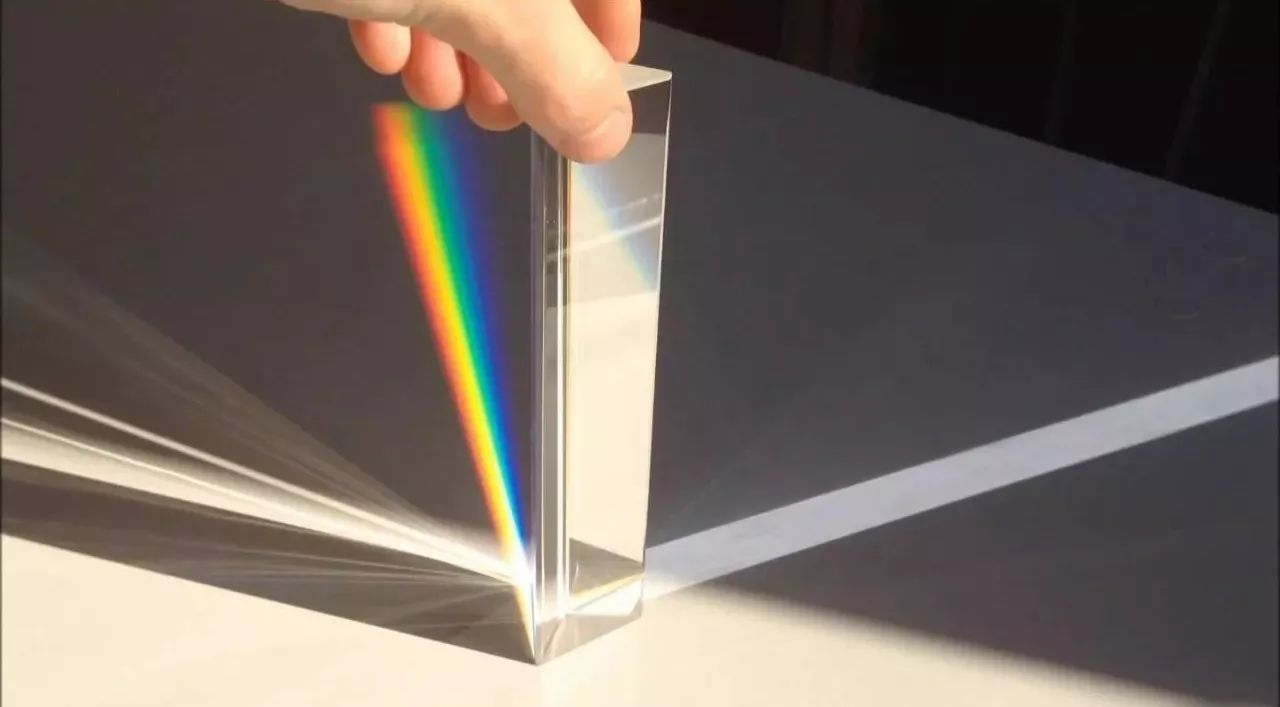
\includegraphics[width=\linewidth]{chap05/dispersion.jpg}
\end{marginfigure}
和\keyindex{干涉}{interference}{}\sidenote{译者注:经典的双缝干涉实验。}
\begin{marginfigure}
    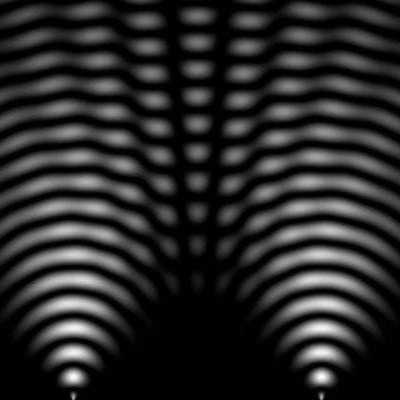
\includegraphics[width=\linewidth]{chap05/interference.jpg}
\end{marginfigure}
等效应建模。
在更精细的细节层面上,需要\keyindex{量子力学}{quantum mechanics}{}来描述光与原子的交互。
幸运的是,解决计算机图形学中的渲染问题不用直接模拟量子力学原理,
故避免了此类方法的复杂性。

在pbrt中,我们将假设几何光学是足够用来描述光与光散射的模型。
这导出了一些整个系统中隐含使用的关于光的行为的基本假设:
\begin{itemize}
    \item \keyindex{线性关系}{linearity}{}:光学系统两个输入的共同效应总是等于每个输入各自效应之和。
    \item \keyindex{能量守恒}{conservation of energy}{}\sidenote{译者注:原文写作energy conservation。}:
    当光从表面或介质散射时,触发的散射不会比它开始时产生更多的能量。
    \item {\sffamily 无偏振}:我们将忽略电磁场的偏振;
    因此,光的唯一相关属性是它关于波长(或等价地,\keyindex{频率}{frequency}{})的分布。
    \item {\sffamily 无}\keyindex{荧光}{fluorescence}{}或\keyindex{磷光}{phosphorescence}{}:
    某一波长的光的行为完全独立于其他波长或时间的光的行为。
    像偏振那样,要包含这些效应并不难,但它们为系统增加的实用价值相对较低。
    \item \keyindex{稳态}{steady state}{}:假设环境中的光达到平衡,
    所以其辐射分布不随时间变化。在现实场景中这对于光几乎是一瞬间发生的,
    所以在实践中这没什么限制。注意磷光也违反了稳态假设。
\end{itemize}

采用几何光学模型最明显的损失是很难考虑\keyindex{衍射}{diffraction}{}和干涉效应。
如\citet[p. 24]{PREISENDORFER19653}所述,这是个很难解决的问题,
例如,当存在这些效应时两区域的总通量不一定等于每个区域各自接收的功率之和。

\subsection{基本量}\label{sub:基本量}
有四个辐射度量数量\sidenote{译者注:依据中国国家标准GB 3102.6-93,
这些量的名称大都可以省略“射”字,例如“辐射出射度”也可以称作
“辐射出度”“辐出射度”“辐出度”,以此类推。后续译文将视情况使用全称或简称。}
是渲染的核心:\keyindex{通量}{flux}{}、
\keyindex{辐射照度}{irradiance}{}/\keyindex{辐射出射度}{radiant exitance}{}、
\keyindex{强度}{intensity}{}和\keyindex{辐射亮度}{radiance}{}。
它们每个都可以从能量(单位为焦耳)依次对时间、面积和方向取极限推导出来。
所有这些辐射度量数量一般都依赖于波长。
对于本章的剩余部分,我们不再明确这一依赖关系,但记住这一性质是很重要的。

\subsubsection*{能量}
我们的起点是\keyindex{能量}{energy}{}
\sidenote{译者注:也称为\keyindex{辐射能}{radiant energy}{}。},
单位为\keyindex{焦耳}{joule}{}(焦,J)
\sidenote{译者注:{\normalfont $1\text{J}=1\text{kg}\cdot\text{m}^2/\text{s}^2$。}}。
照射源发射\keyindex{光子}{photon}{},
每个光子有特定波长并携带特定数量的能量。
所有这些基本辐射度量数量实际都是对光子的不同度量。
波长为$\lambda$的一个光子携带能量为
\begin{align*}
    Q=\frac{hc}{\lambda}\, ,
\end{align*}
其中$c$是光的速率
\sidenote{译者注:指真空环境下的光速;
原文写作{\normalfont $299,472,458\text{m}/\text{s}$},此处更正为国际标准值。}
即$299,792,458\text{m}/\text{s}$,$h$为\keyindex{普朗克常数}{Planck constant}{}
\sidenote{译者注:其单位可化简为{\normalfont$\text{J}\cdot\text{s}$}。},
$h\approx6.626\times10^{-34}\text{kg}\cdot\text{m}^2/\text{s}$。

\subsubsection*{通量}
能量度量了一段时间上的\keyindex{功}{work}{},
尽管渲染一般使用稳态假设,但我们最感兴趣的是度量一瞬间的光。
\keyindex{辐射能通量}{radiant energy flux}{}
\sidenote{译者注:也称辐射通量、辐通量;原文写作radiant flux。},
也称为\keyindex{辐射功率}{radiant power}{}\sidenote{译者注:原文写作power。},
是单位时间内穿过表面或空间区域的能量总量。
辐射通量可以通过求每个微分时间内微分能量的极限算出:
\begin{align*}
    \varPhi=\lim\limits_{\Delta t\rightarrow 0}{\frac{\Delta Q}{\Delta t}}=\frac{\mathrm{d}Q}{\mathrm{d}t}\, .
\end{align*}
它的单位是焦耳$/$秒,即更常见的\keyindex{瓦特}{watt}{}(瓦,W)。

例如,设一光源在一小时内发射了$Q=200,000\text{J}$,
如果这一小时内任何时候发射的能量都相同,
我们可以求得该光源的通量为
\begin{align*}
    \varPhi=200,000\text{J}/3600\text{s}\approx 55.6\text{W}\, .
\end{align*}

反之,设通量是时间的函数,我们可以在一段时间上积分算出总能量:
\begin{align*}
    Q=\int_{t_0}^{t_1}\varPhi(t)\mathrm{d}t\, .
\end{align*}

注意这里我们的记号有些不正式:在其他问题中,因为光子实际上是离散量子,
对趋近于零的微分时间取极限没有实际意义。
但对于渲染目的,光子数量相比于我们感兴趣的度量是巨大的,在实践中这一细节不会有问题。

来自光源的总辐射一般用通量描述。
\reffig{5.6}展示了来自一个点光源的通量由
穿过包围该光源的假想球面的能量总量度量。
注意\reffig{5.6}中在两个球面的任意一个上度量的通量总量是一样的——
尽管穿过大球任意局部的能量比小球少,
但大球的面积更大,意味着总通量一样多。
\begin{figure}[htbp]
    \centering%LaTeX with PSTricks extensions
%%Creator: Inkscape 1.0.1 (3bc2e813f5, 2020-09-07)
%%Please note this file requires PSTricks extensions
\psset{xunit=.5pt,yunit=.5pt,runit=.5pt}
\begin{pspicture}(254.8999939,254.8999939)
{
\newrgbcolor{curcolor}{0 0 0}
\pscustom[linewidth=1,linecolor=curcolor]
{
\newpath
\moveto(188.40000153,127.20999146)
\curveto(188.40000153,151.66779751)(173.6668771,173.71750129)(151.07121577,183.07656872)
\curveto(128.47560051,192.43561706)(102.46763049,187.26077332)(85.17342447,169.96656729)
\curveto(67.87921844,152.67236127)(62.7043747,126.66439125)(72.06342304,104.06877599)
\curveto(81.42249047,81.47311466)(103.47219425,66.73999023)(127.93000031,66.73999023)
\curveto(152.38780636,66.73999023)(174.43751014,81.47311466)(183.79657757,104.06877599)
\curveto(193.15562591,126.66439125)(187.98078217,152.67236127)(170.68657615,169.96656729)
\curveto(153.39237012,187.26077332)(127.3844001,192.43561706)(104.78878484,183.07656872)
\curveto(82.19312351,173.71750129)(67.45999908,151.66779751)(67.45999908,127.20999146)
\curveto(67.45999908,102.7521854)(82.19312351,80.70248162)(104.78878484,71.34341419)
\curveto(127.3844001,61.98436585)(153.39237012,67.15920959)(170.68657615,84.45341562)
\curveto(187.98078217,101.74762164)(193.15562591,127.75559166)(183.79657757,150.35120692)
\curveto(174.43751014,172.94686825)(152.38780636,187.67999268)(127.93000031,187.67999268)
\curveto(103.47219425,187.67999268)(81.42249047,172.94686825)(72.06342304,150.35120692)
\curveto(62.7043747,127.75559166)(67.87921844,101.74762164)(85.17342447,84.45341562)
\curveto(102.46763049,67.15920959)(128.47560051,61.98436585)(151.07121577,71.34341419)
\curveto(173.6668771,80.70248162)(188.40000153,102.7521854)(188.40000153,127.20999146)
\closepath
}
}
{
\newrgbcolor{curcolor}{0 0 0}
\pscustom[linewidth=1,linecolor=curcolor]
{
\newpath
\moveto(254.3999939,127.44999695)
\curveto(254.3999939,178.7964223)(223.46944879,225.08730657)(176.03238777,244.73562073)
\curveto(128.59542349,264.38389481)(73.99460246,253.5198898)(37.68735328,217.21264062)
\curveto(1.3801041,180.90539144)(-9.48390091,126.30457041)(10.16437317,78.86760613)
\curveto(29.81268733,31.43054511)(76.1035716,0.5)(127.44999695,0.5)
\curveto(178.7964223,0.5)(225.08730657,31.43054511)(244.73562073,78.86760613)
\curveto(264.38389481,126.30457041)(253.5198898,180.90539144)(217.21264062,217.21264062)
\curveto(180.90539144,253.5198898)(126.30457041,264.38389481)(78.86760613,244.73562073)
\curveto(31.43054511,225.08730657)(0.5,178.7964223)(0.5,127.44999695)
\curveto(0.5,76.1035716)(31.43054511,29.81268733)(78.86760613,10.16437317)
\curveto(126.30457041,-9.48390091)(180.90539144,1.3801041)(217.21264062,37.68735328)
\curveto(253.5198898,73.99460246)(264.38389481,128.59542349)(244.73562073,176.03238777)
\curveto(225.08730657,223.46944879)(178.7964223,254.3999939)(127.44999695,254.3999939)
\curveto(76.1035716,254.3999939)(29.81268733,223.46944879)(10.16437317,176.03238777)
\curveto(-9.48390091,128.59542349)(1.3801041,73.99460246)(37.68735328,37.68735328)
\curveto(73.99460246,1.3801041)(128.59542349,-9.48390091)(176.03238777,10.16437317)
\curveto(223.46944879,29.81268733)(254.3999939,76.1035716)(254.3999939,127.44999695)
\closepath
}
}
{
\newrgbcolor{curcolor}{0.98823529 0.93333334 0.12941177}
\pscustom[linestyle=none,fillstyle=solid,fillcolor=curcolor]
{
\newpath
\moveto(132.21,146.9699939)
\lineto(130.63,137.2899939)
\lineto(135.58,145.7499939)
\lineto(132.25,136.5299939)
\lineto(138.67,143.9399939)
\lineto(133.71,135.4899939)
\lineto(141.38,141.5799939)
\lineto(134.95,134.1899939)
\lineto(143.61,138.7699939)
\lineto(135.93,132.6899939)
\lineto(145.29,135.5999939)
\lineto(136.62,131.0299939)
\lineto(146.35,132.1799939)
\lineto(136.99,129.2799939)
\lineto(146.77,128.6099939)
\lineto(137.03,127.4799939)
\lineto(146.52,125.0399939)
\lineto(136.74,125.7099939)
\lineto(145.62,121.5599939)
\lineto(136.14,124.0299939)
\lineto(144.1,118.3099939)
\lineto(135.23,122.4799939)
\lineto(142.01,115.3999939)
\lineto(134.05,121.1299939)
\lineto(139.42,112.9199939)
\lineto(132.65,120.0099939)
\lineto(136.41,110.9599939)
\lineto(131.06,119.1699939)
\lineto(133.1,109.5899939)
\lineto(129.35,118.6399939)
\lineto(129.59,108.8399939)
\lineto(127.57,118.4299939)
\lineto(126,108.7599939)
\lineto(125.78,118.5599939)
\lineto(122.47,109.3299939)
\lineto(124.04,118.9999939)
\lineto(119.09,110.5499939)
\lineto(122.42,119.7699939)
\lineto(116,112.3599939)
\lineto(120.96,120.8099939)
\lineto(113.29,114.7099939)
\lineto(119.72,122.1099939)
\lineto(111.06,117.5199939)
\lineto(118.74,123.6099939)
\lineto(109.38,120.6999939)
\lineto(118.05,125.2699939)
\lineto(108.32,124.1199939)
\lineto(117.68,127.0199939)
\lineto(107.9,127.6799939)
\lineto(117.64,128.8099939)
\lineto(108.15,131.2599939)
\lineto(117.93,130.5799939)
\lineto(109.05,134.7299939)
\lineto(118.53,132.2699939)
\lineto(110.57,137.9799939)
\lineto(119.44,133.8199939)
\lineto(112.66,140.8999939)
\lineto(120.62,135.1699939)
\lineto(115.25,143.3699939)
\lineto(122.02,136.2899939)
\lineto(118.26,145.3399939)
\lineto(123.61,137.1199939)
\lineto(121.57,146.7099939)
\lineto(125.32,137.6599939)
\lineto(125.08,147.4599939)
\lineto(127.1,137.8699939)
\lineto(128.66,147.5399939)
\lineto(128.89,137.7399939)
\closepath
}
}
{
\newrgbcolor{curcolor}{0 0 0}
\pscustom[linewidth=0.30000001,linecolor=curcolor]
{
\newpath
\moveto(132.21,146.9699939)
\lineto(130.63,137.2899939)
\lineto(135.58,145.7499939)
\lineto(132.25,136.5299939)
\lineto(138.67,143.9399939)
\lineto(133.71,135.4899939)
\lineto(141.38,141.5799939)
\lineto(134.95,134.1899939)
\lineto(143.61,138.7699939)
\lineto(135.93,132.6899939)
\lineto(145.29,135.5999939)
\lineto(136.62,131.0299939)
\lineto(146.35,132.1799939)
\lineto(136.99,129.2799939)
\lineto(146.77,128.6099939)
\lineto(137.03,127.4799939)
\lineto(146.52,125.0399939)
\lineto(136.74,125.7099939)
\lineto(145.62,121.5599939)
\lineto(136.14,124.0299939)
\lineto(144.1,118.3099939)
\lineto(135.23,122.4799939)
\lineto(142.01,115.3999939)
\lineto(134.05,121.1299939)
\lineto(139.42,112.9199939)
\lineto(132.65,120.0099939)
\lineto(136.41,110.9599939)
\lineto(131.06,119.1699939)
\lineto(133.1,109.5899939)
\lineto(129.35,118.6399939)
\lineto(129.59,108.8399939)
\lineto(127.57,118.4299939)
\lineto(126,108.7599939)
\lineto(125.78,118.5599939)
\lineto(122.47,109.3299939)
\lineto(124.04,118.9999939)
\lineto(119.09,110.5499939)
\lineto(122.42,119.7699939)
\lineto(116,112.3599939)
\lineto(120.96,120.8099939)
\lineto(113.29,114.7099939)
\lineto(119.72,122.1099939)
\lineto(111.06,117.5199939)
\lineto(118.74,123.6099939)
\lineto(109.38,120.6999939)
\lineto(118.05,125.2699939)
\lineto(108.32,124.1199939)
\lineto(117.68,127.0199939)
\lineto(107.9,127.6799939)
\lineto(117.64,128.8099939)
\lineto(108.15,131.2599939)
\lineto(117.93,130.5799939)
\lineto(109.05,134.7299939)
\lineto(118.53,132.2699939)
\lineto(110.57,137.9799939)
\lineto(119.44,133.8199939)
\lineto(112.66,140.8999939)
\lineto(120.62,135.1699939)
\lineto(115.25,143.3699939)
\lineto(122.02,136.2899939)
\lineto(118.26,145.3399939)
\lineto(123.61,137.1199939)
\lineto(121.57,146.7099939)
\lineto(125.32,137.6599939)
\lineto(125.08,147.4599939)
\lineto(127.1,137.8699939)
\lineto(128.66,147.5399939)
\lineto(128.89,137.7399939)
\closepath
}
}
{
\newrgbcolor{curcolor}{0 0 0}
\pscustom[linewidth=1,linecolor=curcolor]
{
\newpath
\moveto(127.12999725,173.73999023)
\lineto(127.12999725,153.51999664)
}
}
{
\newrgbcolor{curcolor}{0 0 0}
\pscustom[linestyle=none,fillstyle=solid,fillcolor=curcolor]
{
\newpath
\moveto(121.63,168.8399939)
\lineto(127.13,173.0899939)
\lineto(132.63,168.8399939)
\lineto(127.13,181.8499939)
\closepath
}
}
{
\newrgbcolor{curcolor}{0.65098041 0.65098041 0.65098041}
\pscustom[linestyle=none,fillstyle=solid,fillcolor=curcolor]
{
\newpath
\moveto(122.83,170.3899939)
\lineto(127.13,180.5399939)
\lineto(127.13,173.7299939)
\closepath
}
}
{
\newrgbcolor{curcolor}{0.40000001 0.40000001 0.40000001}
\pscustom[linestyle=none,fillstyle=solid,fillcolor=curcolor]
{
\newpath
\moveto(131.43,170.3899939)
\lineto(127.13,180.5399939)
\lineto(127.13,173.7299939)
\closepath
}
}
{
\newrgbcolor{curcolor}{0 0 0}
\pscustom[linewidth=1,linecolor=curcolor]
{
\newpath
\moveto(127.12999725,233.55999374)
\lineto(127.12999725,198.08999252)
}
}
{
\newrgbcolor{curcolor}{0 0 0}
\pscustom[linestyle=none,fillstyle=solid,fillcolor=curcolor]
{
\newpath
\moveto(121.63,228.6499939)
\lineto(127.13,232.9099939)
\lineto(132.63,228.6499939)
\lineto(127.13,241.6699939)
\closepath
}
}
{
\newrgbcolor{curcolor}{0.65098041 0.65098041 0.65098041}
\pscustom[linestyle=none,fillstyle=solid,fillcolor=curcolor]
{
\newpath
\moveto(122.83,230.2099939)
\lineto(127.13,240.3499939)
\lineto(127.13,233.5399939)
\closepath
}
}
{
\newrgbcolor{curcolor}{0.40000001 0.40000001 0.40000001}
\pscustom[linestyle=none,fillstyle=solid,fillcolor=curcolor]
{
\newpath
\moveto(131.43,230.2099939)
\lineto(127.13,240.3499939)
\lineto(127.13,233.5399939)
\closepath
}
}
{
\newrgbcolor{curcolor}{0 0 0}
\pscustom[linewidth=1,linecolor=curcolor]
{
\newpath
\moveto(107.52999878,169.63999176)
\lineto(116.30000305,151.42999268)
}
}
{
\newrgbcolor{curcolor}{0 0 0}
\pscustom[linestyle=none,fillstyle=solid,fillcolor=curcolor]
{
\newpath
\moveto(104.7,162.8299939)
\lineto(107.81,169.0599939)
\lineto(114.62,167.6099939)
\lineto(104.01,176.9499939)
\closepath
}
}
{
\newrgbcolor{curcolor}{0.65098041 0.65098041 0.65098041}
\pscustom[linestyle=none,fillstyle=solid,fillcolor=curcolor]
{
\newpath
\moveto(105.11,164.7599939)
\lineto(104.58,175.7599939)
\lineto(107.54,169.6299939)
\closepath
}
}
{
\newrgbcolor{curcolor}{0.40000001 0.40000001 0.40000001}
\pscustom[linestyle=none,fillstyle=solid,fillcolor=curcolor]
{
\newpath
\moveto(112.85,168.4899939)
\lineto(104.58,175.7599939)
\lineto(107.54,169.6299939)
\closepath
}
}
{
\newrgbcolor{curcolor}{0 0 0}
\pscustom[linewidth=1,linecolor=curcolor]
{
\newpath
\moveto(81.55999756,223.53999329)
\lineto(96.95999908,191.5799942)
}
}
{
\newrgbcolor{curcolor}{0 0 0}
\pscustom[linestyle=none,fillstyle=solid,fillcolor=curcolor]
{
\newpath
\moveto(78.74,216.7199939)
\lineto(81.85,222.9499939)
\lineto(88.65,221.4999939)
\lineto(78.05,230.8299939)
\closepath
}
}
{
\newrgbcolor{curcolor}{0.65098041 0.65098041 0.65098041}
\pscustom[linestyle=none,fillstyle=solid,fillcolor=curcolor]
{
\newpath
\moveto(79.14,218.6499939)
\lineto(78.62,229.6499939)
\lineto(81.57,223.5199939)
\closepath
}
}
{
\newrgbcolor{curcolor}{0.40000001 0.40000001 0.40000001}
\pscustom[linestyle=none,fillstyle=solid,fillcolor=curcolor]
{
\newpath
\moveto(86.89,222.3799939)
\lineto(78.62,229.6499939)
\lineto(81.57,223.5199939)
\closepath
}
}
{
\newrgbcolor{curcolor}{0 0 0}
\pscustom[linewidth=1,linecolor=curcolor]
{
\newpath
\moveto(92.12999725,156.56999207)
\lineto(107.69999695,143.66999054)
}
}
{
\newrgbcolor{curcolor}{0 0 0}
\pscustom[linestyle=none,fillstyle=solid,fillcolor=curcolor]
{
\newpath
\moveto(92.4,149.1999939)
\lineto(92.63,156.1599939)
\lineto(99.42,157.6799939)
\lineto(85.89,161.7399939)
\closepath
}
}
{
\newrgbcolor{curcolor}{0.65098041 0.65098041 0.65098041}
\pscustom[linestyle=none,fillstyle=solid,fillcolor=curcolor]
{
\newpath
\moveto(91.97,151.1199939)
\lineto(86.9,160.9099939)
\lineto(92.15,156.5599939)
\closepath
}
}
{
\newrgbcolor{curcolor}{0.40000001 0.40000001 0.40000001}
\pscustom[linestyle=none,fillstyle=solid,fillcolor=curcolor]
{
\newpath
\moveto(97.45,157.7399939)
\lineto(86.9,160.9099939)
\lineto(92.15,156.5599939)
\closepath
}
}
{
\newrgbcolor{curcolor}{0 0 0}
\pscustom[linewidth=1,linecolor=curcolor]
{
\newpath
\moveto(46.06999969,194.73999405)
\lineto(73.38999939,172.10999298)
}
}
{
\newrgbcolor{curcolor}{0 0 0}
\pscustom[linestyle=none,fillstyle=solid,fillcolor=curcolor]
{
\newpath
\moveto(46.34,187.3699939)
\lineto(46.57,194.3299939)
\lineto(53.37,195.8499939)
\lineto(39.83,199.9199939)
\closepath
}
}
{
\newrgbcolor{curcolor}{0.65098041 0.65098041 0.65098041}
\pscustom[linestyle=none,fillstyle=solid,fillcolor=curcolor]
{
\newpath
\moveto(45.91,189.2899939)
\lineto(40.84,199.0799939)
\lineto(46.09,194.7299939)
\closepath
}
}
{
\newrgbcolor{curcolor}{0.40000001 0.40000001 0.40000001}
\pscustom[linestyle=none,fillstyle=solid,fillcolor=curcolor]
{
\newpath
\moveto(51.4,195.9099939)
\lineto(40.84,199.0799939)
\lineto(46.09,194.7299939)
\closepath
}
}
{
\newrgbcolor{curcolor}{0 0 0}
\pscustom[linewidth=1,linecolor=curcolor]
{
\newpath
\moveto(147.63000488,169.3299942)
\lineto(138.8500061,151.11999512)
}
}
{
\newrgbcolor{curcolor}{0 0 0}
\pscustom[linestyle=none,fillstyle=solid,fillcolor=curcolor]
{
\newpath
\moveto(140.54,167.2999939)
\lineto(147.34,168.7499939)
\lineto(150.45,162.5199939)
\lineto(151.14,176.6299939)
\closepath
}
}
{
\newrgbcolor{curcolor}{0.65098041 0.65098041 0.65098041}
\pscustom[linestyle=none,fillstyle=solid,fillcolor=curcolor]
{
\newpath
\moveto(142.3,168.1799939)
\lineto(150.57,175.4499939)
\lineto(147.62,169.3199939)
\closepath
}
}
{
\newrgbcolor{curcolor}{0.40000001 0.40000001 0.40000001}
\pscustom[linestyle=none,fillstyle=solid,fillcolor=curcolor]
{
\newpath
\moveto(150.04,164.4499939)
\lineto(150.57,175.4499939)
\lineto(147.62,169.3199939)
\closepath
}
}
{
\newrgbcolor{curcolor}{0 0 0}
\pscustom[linewidth=1,linecolor=curcolor]
{
\newpath
\moveto(173.58999634,223.21999359)
\lineto(158.19000244,191.26999283)
}
}
{
\newrgbcolor{curcolor}{0 0 0}
\pscustom[linestyle=none,fillstyle=solid,fillcolor=curcolor]
{
\newpath
\moveto(166.5,221.1899939)
\lineto(173.31,222.6399939)
\lineto(176.42,216.4099939)
\lineto(177.11,230.5199939)
\closepath
}
}
{
\newrgbcolor{curcolor}{0.65098041 0.65098041 0.65098041}
\pscustom[linestyle=none,fillstyle=solid,fillcolor=curcolor]
{
\newpath
\moveto(168.26,222.0699939)
\lineto(176.54,229.3399939)
\lineto(173.58,223.2099939)
\closepath
}
}
{
\newrgbcolor{curcolor}{0.40000001 0.40000001 0.40000001}
\pscustom[linestyle=none,fillstyle=solid,fillcolor=curcolor]
{
\newpath
\moveto(176.01,218.3399939)
\lineto(176.54,229.3399939)
\lineto(173.58,223.2099939)
\closepath
}
}
{
\newrgbcolor{curcolor}{0 0 0}
\pscustom[linewidth=1,linecolor=curcolor]
{
\newpath
\moveto(163.02000427,156.25999451)
\lineto(147.44999695,143.35999298)
}
}
{
\newrgbcolor{curcolor}{0 0 0}
\pscustom[linestyle=none,fillstyle=solid,fillcolor=curcolor]
{
\newpath
\moveto(155.73,157.3699939)
\lineto(162.52,155.8499939)
\lineto(162.75,148.8899939)
\lineto(169.26,161.4299939)
\closepath
}
}
{
\newrgbcolor{curcolor}{0.65098041 0.65098041 0.65098041}
\pscustom[linestyle=none,fillstyle=solid,fillcolor=curcolor]
{
\newpath
\moveto(157.7,157.4399939)
\lineto(168.25,160.5999939)
\lineto(163.01,156.2499939)
\closepath
}
}
{
\newrgbcolor{curcolor}{0.40000001 0.40000001 0.40000001}
\pscustom[linestyle=none,fillstyle=solid,fillcolor=curcolor]
{
\newpath
\moveto(163.18,150.8199939)
\lineto(168.25,160.5999939)
\lineto(163.01,156.2499939)
\closepath
}
}
{
\newrgbcolor{curcolor}{0 0 0}
\pscustom[linewidth=1,linecolor=curcolor]
{
\newpath
\moveto(209.08000183,194.42999268)
\lineto(181.77000427,171.79999542)
}
}
{
\newrgbcolor{curcolor}{0 0 0}
\pscustom[linestyle=none,fillstyle=solid,fillcolor=curcolor]
{
\newpath
\moveto(201.79,195.5399939)
\lineto(208.58,194.0199939)
\lineto(208.81,187.0599939)
\lineto(215.32,199.5999939)
\closepath
}
}
{
\newrgbcolor{curcolor}{0.65098041 0.65098041 0.65098041}
\pscustom[linestyle=none,fillstyle=solid,fillcolor=curcolor]
{
\newpath
\moveto(203.75,195.6099939)
\lineto(214.31,198.7699939)
\lineto(209.06,194.4199939)
\closepath
}
}
{
\newrgbcolor{curcolor}{0.40000001 0.40000001 0.40000001}
\pscustom[linestyle=none,fillstyle=solid,fillcolor=curcolor]
{
\newpath
\moveto(209.24,188.9799939)
\lineto(214.31,198.7699939)
\lineto(209.06,194.4199939)
\closepath
}
}
\end{pspicture}

    \caption{辐射通量$\varPhi$度量穿过表面或空间区域的能量。
    这里来自一个点光源的通量由包围它的球来度量。}
    \label{fig:5.6}
\end{figure}

\subsubsection*{辐射照度与辐射出射度}

\subsection{亮度和光度学}\label{sub:亮度和光度学}

\section{表面反射}\label{sec:表面反射}

当光入射到表面时,表面会散射该光,将其一部分反射回环境中。
有两个需要描述的效应以对反射建模:反射光的光谱分布和其方向分布。
例如,柠檬皮大都吸收了蓝波长的光而反射了大部分红和绿波长的光
(回想\reffig{5.1}中柠檬皮的反射SPD)。
因此,当用白光照射它时,其颜色是黄色。
无论从哪个方向观察,皮的颜色都相当一致,
但有的方向会有\keyindex{高光}{highlight}{}——会看见与其说黄色不如说白色的更亮区域
\sidenote{译者注:有高光区的柠檬照片。}。
\begin{marginfigure}
    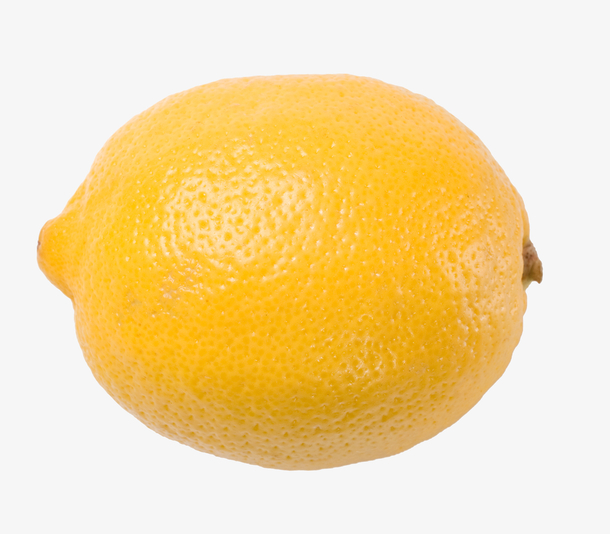
\includegraphics[width=\linewidth]{chap05/lemon.jpg}
\end{marginfigure}
相反,镜子一点反射的光几乎完全取决于观察方向。
在镜子的固定点上,当观察角度变化时,镜子反射的物体也随之变化。

来自\keyindex{半透明}{translucent}{}表面的反射更复杂;
从皮和叶子到蜡和液体的各种材料都
表现出\keyindex{次表面光传输}{subsurface light transport}{light transport光传输},
即进入表面一点的光在有一定距离的地方退出。
(例如考虑在一个人的嘴巴里开手电筒会让他的脸颊被照亮,
因为进入脸颊内侧的光穿过了皮肤并从脸上退出。)

有两种抽象来为光的反射描述这些机制:
\refsub{BRDF}和\refsub{BSSRDF}分别介绍的BRDF和BSSRDF。
BRDF描述一点的表面反射而忽略次表面光传输效应;
对于不受该传输机制明显影响的材料,
这一简化会减少报错并让渲染算法的实现高效得多。
BSSRDF推广了BRDF并描述来自半透明材料光反射的更一般设置。

\subsection{BRDF}\label{sub:BRDF}
\keyindex{双向反射分布函数}{bidirectional reflectance distribution function}{}(BRDF)
为描述来自表面的反射给出了形式。考虑\reffig{5.18}中的设置:
我们想知道,作为沿方向${\bm\omega}_{\mathrm{i}}$
入射辐亮度$L_{\mathrm{i}}({\bm p},{\bm\omega}_{\mathrm{i}})$的结果,
在朝向观察者的方向${\bm\omega}_{\mathrm{o}}$中
有多少辐射亮度$L_{\mathrm{o}}({\bm p},{\bm\omega}_{\mathrm{o}})$离开表面。
\begin{figure}[htbp]
    \centering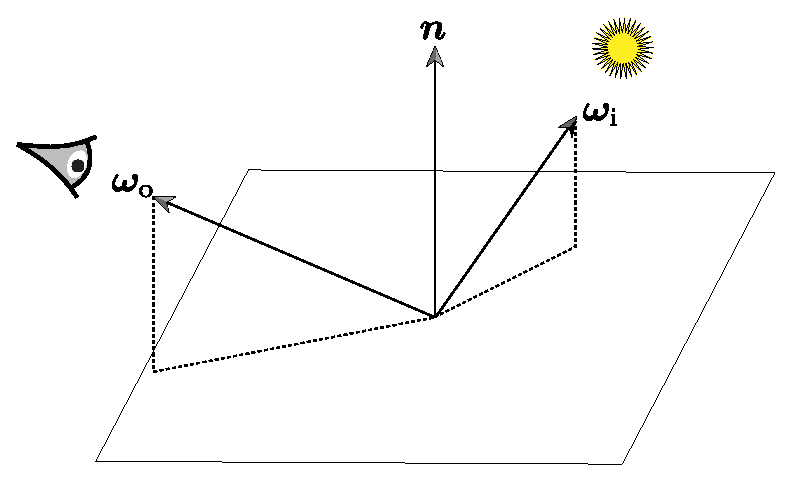
\includegraphics[width=0.5\linewidth]{chap05/BRDF.eps}
    \caption{BRDF。双向反射分布函数是在一对方向${\bm\omega}_{\mathrm{i}}$
        和${\bm\omega}_{\mathrm{o}}$上描述有多少沿${\bm\omega}_{\mathrm{i}}$
        入射的光从表面朝方向${\bm\omega}_{\mathrm{o}}$散射的4D函数。}
    \label{fig:5.18}
\end{figure}

如果方向${\bm\omega}_{\mathrm{i}}$视作方向的微分锥,则$\bm p$处的微分辐照度是
\begin{align}\label{eq:5.7}
    \mathrm{d}E({\bm p},{\bm\omega}_{\mathrm{i}})=L_{\mathrm{i}}({\bm p},{\bm\omega}_{\mathrm{i}})\cos\theta_{\mathrm{i}}\mathrm{d}{\bm\omega}_{\mathrm{i}}\, .
\end{align}

要被反射到方向${\bm\omega}_{\mathrm{o}}$的辐射亮度微分量取决于该辐射照度。
因为几何光学的线性假设,反射的微分辐射亮度正比于辐射照度
\begin{align*}
    \mathrm{d}L_{\mathrm{o}}({\bm p},{\bm\omega}_{\mathrm{o}})\propto\mathrm{d}E({\bm p},{\bm\omega}_{\mathrm{i}})\, .
\end{align*}

比例常数为这对特定方向${\bm\omega}_{\mathrm{i}}$和${\bm\omega}_{\mathrm{o}}$定义了曲面的BRDF:
\begin{align}\label{eq:5.8}
    f_{\mathrm{r}}({\bm p},{\bm \omega}_\mathrm{o},{\bm \omega}_\mathrm{i})=\frac{\mathrm{d}L_{\mathrm{o}}({\bm p},{\bm\omega}_{\mathrm{o}})}{\mathrm{d}E({\bm p},{\bm\omega}_{\mathrm{i}})}=\frac{\mathrm{d}L_{\mathrm{o}}({\bm p},{\bm\omega}_{\mathrm{o}})}{L_{\mathrm{i}}({\bm p},{\bm\omega}_{\mathrm{i}})\cos\theta_{\mathrm{i}}\mathrm{d}{\bm\omega}_{\mathrm{i}}}\, .
\end{align}

基于物理的BRDF有两个重要性质:
\begin{enumerate}
    \item \keyindex{互易性}{reciprocity}{}:对所有方向对${\bm\omega}_{\mathrm{i}}$和${\bm\omega}_{\mathrm{o}}$,
          $f_{\mathrm{r}}({\bm p},{\bm \omega}_\mathrm{i},{\bm \omega}_\mathrm{o})=f_{\mathrm{r}}({\bm p},{\bm \omega}_\mathrm{o},{\bm \omega}_\mathrm{i})$。
    \item {\sffamily 能量守恒}:光反射的总能量少于或等于入射光的能量。
          对于所有方向${\bm\omega}_{\mathrm{o}}$,
          \begin{align*}
              \int\limits_{H^2({\bm n})}f_{\mathrm{r}}({\bm p},{\bm \omega}_\mathrm{o},{\bm \omega}')\cos\theta'\mathrm{d}{\bm\omega}'\le1\, .
          \end{align*}
\end{enumerate}

曲面的\keyindex{双向透射分布函数}{bidirectional transmittance distribution function}{}
(BTDF)描述透射光的分布,可以用和BRDF一样的方法定义。
BTDF一般表示为$f_{\mathrm{t}}({\bm p},{\bm \omega}_\mathrm{o},{\bm \omega}_\mathrm{i})$,
其中${\bm\omega}_{\mathrm{i}}$和${\bm\omega}_{\mathrm{o}}$在绕$\bm p$的相对半球内。
要注意的是,BTDF不遵循上面定义的互异性;
我们将在\refsec{镜面反射与透射}和\refsub{非对称散射}详细讨论该问题。

为了等式的方便,我们把统一考虑时的BRDF和BTDF表示为$f({\bm p},{\bm \omega}_\mathrm{o},{\bm \omega}_\mathrm{i})$;
我们称之为\keyindex{双向散射分布函数}{bidirectional scattering distribution function}{}(BSFD)。
第\refchap{反射模型}将完全专注于描述对渲染有用的各种BSDF。

利用BSDF的定义,我们有
\begin{align*}
    \mathrm{d}L_{\mathrm{o}}({\bm p},{\bm\omega}_{\mathrm{o}})=f({\bm p},{\bm \omega}_\mathrm{o},{\bm \omega}_\mathrm{i})L_{\mathrm{i}}({\bm p},{\bm\omega}_{\mathrm{i}})|\cos\theta_{\mathrm{i}}|\mathrm{d}{\bm\omega}_{\mathrm{i}}\, .
\end{align*}
这里给项$\cos\theta_{\mathrm{i}}$加上了绝对值。
这样做是因为pbrt中曲面法线并没有调整为和${\bm\omega}_{\mathrm{i}}$位于曲面同侧
(许多其他渲染系统都这样做,但我们发现让它们留在原来\refvar{Shape}{}给出的自然朝向会更有用)。
这样做更容易一致地在系统别处运用如“假设曲面法线指向曲面外侧”那样的约定。
因此,像这样给项$\cos\theta_{\mathrm{i}}$加上绝对值保证了实际计算出所需的数量。
我们可以在绕$\bm p$的入射方向球内对该等式积分以计算由于各个方向对$\bm p$的照射
而得到的沿方向${\bm\omega}_{\mathrm{o}}$的出射辐亮度:
\begin{align}\label{eq:5.9}
    L_{\mathrm{o}}({\bm p},{\bm\omega}_{\mathrm{o}})=\int\limits_{S^2}f({\bm p},{\bm \omega}_\mathrm{o},{\bm \omega}_\mathrm{i})L_{\mathrm{i}}({\bm p},{\bm\omega}_{\mathrm{i}})|\cos\theta_{\mathrm{i}}|\mathrm{d}{\bm\omega}_{\mathrm{i}}\, .
\end{align}
这是渲染中的基本方程;它描述了一点的入射光分布
是怎样基于表面的散射性质转化为出射分布的。
当(像这里)球$S^2$作为积分域时它常常称为\keyindex{散射方程}{scattering equation}{},
当只在上半球$H^2({\bm n})$积分时则称\keyindex{反射方程}{reflection equation}{}。
\refchap{光传输I:表面反射}和\refchap{光传输III:双向方法}中积分例程的
关键任务之一就是计算场景中曲面上的点的该积分值。

\subsection{BSSRDF}\label{sub:BSSRDF}
